% Options for packages loaded elsewhere
\PassOptionsToPackage{unicode}{hyperref}
\PassOptionsToPackage{hyphens}{url}
\PassOptionsToPackage{dvipsnames,svgnames*,x11names*}{xcolor}
%
\documentclass[
]{turabian-researchpaper}
\usepackage{lmodern}
\usepackage{amssymb,amsmath}
\usepackage{ifxetex,ifluatex}
\ifnum 0\ifxetex 1\fi\ifluatex 1\fi=0 % if pdftex
  \usepackage[T1]{fontenc}
  \usepackage[utf8]{inputenc}
  \usepackage{textcomp} % provide euro and other symbols
\else % if luatex or xetex
  \usepackage{unicode-math}
  \defaultfontfeatures{Scale=MatchLowercase}
  \defaultfontfeatures[\rmfamily]{Ligatures=TeX,Scale=1}
\fi
% Use upquote if available, for straight quotes in verbatim environments
\IfFileExists{upquote.sty}{\usepackage{upquote}}{}
\IfFileExists{microtype.sty}{% use microtype if available
  \usepackage[]{microtype}
  \UseMicrotypeSet[protrusion]{basicmath} % disable protrusion for tt fonts
}{}
\makeatletter
\@ifundefined{KOMAClassName}{% if non-KOMA class
  \IfFileExists{parskip.sty}{%
    \usepackage{parskip}
  }{% else
    \setlength{\parindent}{0pt}
    \setlength{\parskip}{6pt plus 2pt minus 1pt}}
}{% if KOMA class
  \KOMAoptions{parskip=half}}
\makeatother
\usepackage{xcolor}
\IfFileExists{xurl.sty}{\usepackage{xurl}}{} % add URL line breaks if available
\IfFileExists{bookmark.sty}{\usepackage{bookmark}}{\usepackage{hyperref}}
\hypersetup{
  pdftitle={Hebrew GRAMMAR Quest},
  pdfauthor={Chris Flanagan},
  colorlinks=true,
  linkcolor=Maroon,
  filecolor=Maroon,
  citecolor=Blue,
  urlcolor=Blue,
  pdfcreator={LaTeX via pandoc}}
\urlstyle{same} % disable monospaced font for URLs
\usepackage{longtable,booktabs}
% Correct order of tables after \paragraph or \subparagraph
\usepackage{etoolbox}
\makeatletter
\patchcmd\longtable{\par}{\if@noskipsec\mbox{}\fi\par}{}{}
\makeatother
% Allow footnotes in longtable head/foot
\IfFileExists{footnotehyper.sty}{\usepackage{footnotehyper}}{\usepackage{footnote}}
\makesavenoteenv{longtable}
\usepackage{graphicx}
\makeatletter
\def\maxwidth{\ifdim\Gin@nat@width>\linewidth\linewidth\else\Gin@nat@width\fi}
\def\maxheight{\ifdim\Gin@nat@height>\textheight\textheight\else\Gin@nat@height\fi}
\makeatother
% Scale images if necessary, so that they will not overflow the page
% margins by default, and it is still possible to overwrite the defaults
% using explicit options in \includegraphics[width, height, ...]{}
\setkeys{Gin}{width=\maxwidth,height=\maxheight,keepaspectratio}
% Set default figure placement to htbp
\makeatletter
\def\fps@figure{htbp}
\makeatother
\setlength{\emergencystretch}{3em} % prevent overfull lines
\providecommand{\tightlist}{%
  \setlength{\itemsep}{0pt}\setlength{\parskip}{0pt}}
\setcounter{secnumdepth}{5}
\usepackage{booktabs}
\usepackage{pdfpages}
\usepackage[]{natbib}
\bibliographystyle{turabian}

\title{Hebrew GRAMMAR Quest}
\author{Chris Flanagan}
\date{2020-10-19}

\begin{document}
\maketitle

{
\hypersetup{linkcolor=}
\setcounter{tocdepth}{2}
\tableofcontents
}
\listoftables
\listoffigures
\hypertarget{biblical-hebrew-grammar-the-holy-language-way}{%
\section*{Biblical Hebrew Grammar, the Holy Language way}\label{biblical-hebrew-grammar-the-holy-language-way}}
\addcontentsline{toc}{section}{Biblical Hebrew Grammar, the Holy Language way}

\begin{center}
\includegraphics[width=500pt]{images/hli_cover} \end{center}

\hypertarget{this-is-a-previewdemo-version-of-hebrew-grammar-quest}{%
\section*{This is a Preview/Demo Version of Hebrew GRAMMAR Quest}\label{this-is-a-previewdemo-version-of-hebrew-grammar-quest}}
\addcontentsline{toc}{section}{This is a Preview/Demo Version of Hebrew GRAMMAR Quest}

This book covers the first three of the thirty-five total lessons:

\begin{enumerate}
\def\labelenumi{\arabic{enumi}.}
\tightlist
\item
  The Hebrew Aleph-Bet
\item
  The Hebrew Vowels
\item
  Hebrew syllabification and Pronunciation
\end{enumerate}

In addition, the preface, which outlines our vision for the course, and some Appendices are complete and available.

We have two goals for this version:

\begin{enumerate}
\def\labelenumi{\arabic{enumi}.}
\tightlist
\item
  Create a ``proof of concept'' version for our Holy Language ministry volunteers. We want to gather feedback on content and overall direction before proceeding with development of all 35 lessons.
\item
  Eventually, these three lessons will comprise a ``demo'' version of Hebrew GRAMMAR Quest to be made available to non-subscribers. The goal is that they will see, like and become supporters of Holy Language Institute, giving them access to not only the entire grammar course, but Hebrew Quest and all the other amazing teaching content.
\end{enumerate}

The anticipated full course availability date is Q2 2021.

Thank you in advance for reading these three lessons. Please email errors, omissions, comments, or suggestions to \href{mailto:holylanguagecourses@gmail.com}{\nolinkurl{holylanguagecourses@gmail.com}}

\hypertarget{preface}{%
\section*{Preface: The philosophy of this book and course}\label{preface}}
\addcontentsline{toc}{section}{Preface: The philosophy of this book and course}

\begin{center}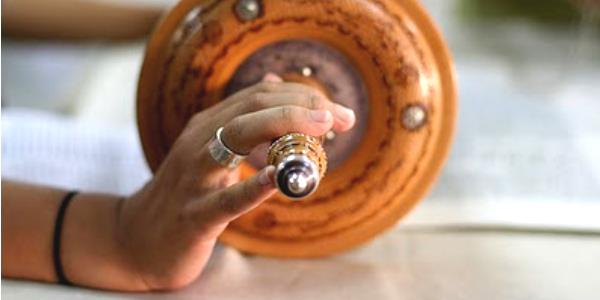
\includegraphics[width=500pt]{images/torah_scroll} \end{center}

Many Hebrew grammar courses and books treat learning God's Holy Language as if it were just another academic exercise. Listen to a lecture, read a chapter, take a test, and you'll learn Hebrew.

We wish it were that simple.

Hebrew, the Holy Language Way, requires \textbf{active} participation.

That's where our Holy Language Learning Philosophy comes in.

\hypertarget{our-learning-philosophy-active-engagement}{%
\subsection*{Our Learning Philosophy = ACTIVE Engagement}\label{our-learning-philosophy-active-engagement}}
\addcontentsline{toc}{subsection}{Our Learning Philosophy = ACTIVE Engagement}

Learning Hebrew the Holy Language Way is designed not just to feed you fish, but to teach you to fish\footnote{Refer to Hebrew Quest, lesson 1.}. When someone feeds you fish, you are only passively receiving. When you learn to fish you are being active; being intentional.

In other words, we believe you will learn best when you actively (and dare we say ``passionately'') \textbf{\emph{engage}} with the Holy Scriptures. If done this way, learning Hebrew will not merely be another academic course you take, but it can be a life-changing experience.

With Hebrew GRAMMAR Quest, Holy Language Institute is offering yet another way for you to actively embrace the Jewishness of our faith.

\hypertarget{relationship-to-hebrew-quest}{%
\subsection*{Relationship to Hebrew Quest}\label{relationship-to-hebrew-quest}}
\addcontentsline{toc}{subsection}{Relationship to Hebrew Quest}

\textbf{\emph{Hebrew Quest}} took you directly \emph{to} the Hebrew Scriptures and brought you in touch with the Hebraic side of the Bible that, perhaps, you had never experienced before. We introduced you to a different aspect of what you may have known as ``the Old Testament.'' Maybe before Hebrew Quest, you had kept this ``Old Testament'' at a safe distance (after all, it was old and you are new!); but now you may have a new appreciation and perhaps you are building a closer friendship with what you now know as the ``Tanach'' or the ``Hebrew Scriptures.''

\textbf{\emph{Hebrew GRAMMAR Quest}} is designed to take you to the next stage of that friendship. It is designed to take you \emph{inside} the Hebrew Scriptures. Maybe it's like progressing from a ``good friend'' to an ``intimate'' friend. A friend for whom you are there during the good and the bad . . . and that friend is there for you offering you wisdom and counsel.

Such a friendship can be challenging, and even difficult at times\footnote{see Philippians 2:12}, but it can also be one of the most rewarding relationships you can have this side of heaven.

Whether or not you have finished (or even started) Hebrew Quest, we believe you will find Hebrew GRAMMAR quest a fruitful and life-changing experience. See \protect\hyperlink{difference}{Appendix Q\&A} for a larger discussion on how Hebrew Quest and Hebrew GRAMMAR Quest work together.

\hypertarget{three-stages-of-preparation}{%
\subsection*{Three Stages of Preparation}\label{three-stages-of-preparation}}
\addcontentsline{toc}{subsection}{Three Stages of Preparation}

According to Dr.~Wayne Stiles, to get the most out of a tour to Israel, one must actively prepare. In fact, there are three stages of preparation Stiles says a traveler must undertake to gain maximum benefit from a Holy Land tour\footnote{Stiles, Wayne. ``How to Prepare for a Holy Land Tour.'' Wayne Stiles. February 20, 2013. \url{https://waynestiles.com/how-to-prepare-for-a-holy-land-tour/}. Accessed September 28, 2020.}

\begin{enumerate}
\def\labelenumi{\arabic{enumi}.}
\tightlist
\item
  Practical Preparation
\item
  Physical Preparation
\item
  Spiritual Preparation
\end{enumerate}

\hypertarget{we-believe-these-exact-principles-apply-to-learning-hebrew-the-holy-language-way}{%
\subsubsection*{We believe these exact principles apply to learning Hebrew the Holy Language way!}\label{we-believe-these-exact-principles-apply-to-learning-hebrew-the-holy-language-way}}
\addcontentsline{toc}{subsubsection}{We believe these exact principles apply to learning Hebrew the Holy Language way!}

Read on for an explanation.

\hypertarget{practical-preparation-the-lay-of-the-hebrew-grammar-land}{%
\subsection*{\texorpdfstring{\emph{Practical} Preparation: The lay of the Hebrew Grammar land}{Practical Preparation: The lay of the Hebrew Grammar land}}\label{practical-preparation-the-lay-of-the-hebrew-grammar-land}}
\addcontentsline{toc}{subsection}{\emph{Practical} Preparation: The lay of the Hebrew Grammar land}

Before the big trip to Israel, you need to know some basics.

\begin{itemize}
\tightlist
\item
  You need some basic Holy Land Geography

  \begin{itemize}
  \tightlist
  \item
    You need some basics as to what happened where
  \item
    This way, you won't be completely lost when you arrive at a specific site, say Capernaum or Mount Carmel
  \item
    You need to know why that place has meaning and is worth your time
  \end{itemize}
\end{itemize}

You might call this ``getting the lay of the land''.

\textbf{Primarily, what this book consists of, is giving you the lay of the Hebrew Grammar land}.

In our application, we will give you ``Seven Practical Points.'' These are the most significant things you will need to know about the lesson.

Most importantly, our goal is to keep this discussion at a high-level. This means, where other textbooks might spend time explaining concepts to you in great detail, we will not. Our goal is to give you just enough to pique your interest and get you pointed in the right direction.

We believe that you will learn best not from reading it in a book or watching a video, but you will learn best by putting concepts into practice.

This is where \emph{physical preparation} comes in. But first, let's talk for a minute about safety . . . your ``syntactical safety!''

\hypertarget{practical-preparation-equipment-check}{%
\subsection*{\texorpdfstring{\emph{Practical} Preparation: Equipment Check}{Practical Preparation: Equipment Check}}\label{practical-preparation-equipment-check}}
\addcontentsline{toc}{subsection}{\emph{Practical} Preparation: Equipment Check}

Each lesson of Hebrew GRAMMAR Quest builds upon the previous one.

At the beginning of each chapter, you will see an Israeli stop sign with a few questions.

\begin{center}
\includegraphics[width=200pt]{images/stopil} \end{center}

Use this as an opportunity to check whether you are familiar enough with the major concepts (and memorization where needed) from the previous lesson before you move on with your journey.

We call this ``Equipment Check.''

Here, we leave the decision to proceed with your quest up to you. Be honest with yourself. If you are unsure about any area, we strongly encourage you to return to Anki for some more review.

\hypertarget{physical-preparation-get-hebrew-healthy-with-anki-aerobics}{%
\subsection*{\texorpdfstring{\emph{Physical} Preparation: Get Hebrew healthy with Anki Aerobics}{Physical Preparation: Get Hebrew healthy with Anki Aerobics}}\label{physical-preparation-get-hebrew-healthy-with-anki-aerobics}}
\addcontentsline{toc}{subsection}{\emph{Physical} Preparation: Get Hebrew healthy with Anki Aerobics}

Israel is a rocky, hilly place. Many of the best sites require some walking, or even a small hike from the parking lot. Those who hope to passively see the country from a bus window but who could have done more had they done some exercising beforehand, are going to miss out on the best parts. For maximum benefit, travelers must be ready for a lot of walking.

Most of your class time will be spent not in reading this book or watching lectures. In Hebrew GRAMMAR Quest, your \textbf{TRUE} learning will take place during what we call ``ACTIVities.''

In fact, we'd like this book to be like be your personal trainer. A trainer shows you how to do your workout safely and effectively. She gives you some ``practical'' pointers and then turns it over to you to do the actual lifting. In our case, your brain will be doing the lifting instead of your biceps.

\begin{itemize}
\tightlist
\item
  The majority of your learning time will be spent in a free flashcard program called Anki. Please see \protect\hyperlink{Anki}{About Anki} for additional information on Anki if you are not familiar with it.

  \begin{itemize}
  \tightlist
  \item
    \textbf{Anki} is the equivalent of your gym and cardio equipment for Hebrew Health
  \item
    Just like working out is not easy and you don't always see quick results, don't expect Anki to be easy or expect to breeze through it
  \item
    Just like physical exercise, if you stick with it, you will see the rewards over time
  \end{itemize}
\item
  In addition to Anki, some lessons will have worksheets to reinforce concepts
\end{itemize}

\hypertarget{download-the-hebrew-grammar-quest-preview-version-anki-deck}{%
\subsubsection*{\texorpdfstring{\href{./images/Hebrew\%20Grammar\%20Quest\%20PREVIEW.apkg}{Download the Hebrew GRAMMAR Quest (Preview Version) Anki Deck}}{Download the Hebrew GRAMMAR Quest (Preview Version) Anki Deck}}\label{download-the-hebrew-grammar-quest-preview-version-anki-deck}}
\addcontentsline{toc}{subsubsection}{\href{./images/Hebrew\%20Grammar\%20Quest\%20PREVIEW.apkg}{Download the Hebrew GRAMMAR Quest (Preview Version) Anki Deck}}

\begin{itemize}
\tightlist
\item
  See \protect\hyperlink{Anki}{Anki discussion in the appendix} for additional information on Anki, including installation and settings
\end{itemize}

\hypertarget{physical-preparation-combat-the-fog-aka-grammar-jet-lag}{%
\subsection*{\texorpdfstring{\emph{Physical} Preparation: Combat ``the fog'' (aka grammar jet lag)}{Physical Preparation: Combat ``the fog'' (aka grammar jet lag)}}\label{physical-preparation-combat-the-fog-aka-grammar-jet-lag}}
\addcontentsline{toc}{subsection}{\emph{Physical} Preparation: Combat ``the fog'' (aka grammar jet lag)}

For most of us, Israel is close to halfway around the globe away from home. After such a long flight, we are unlikely to completely avoid jet lag, but we can take steps to minimize the effects and work through it as quickly as possible.

Jet lag is similar to a phenomenon we can encounter when we undertake a study of a new language. Dr.~Bill Mounce calls "the fog.'

\begin{itemize}
\item
  Many times, things won't make sense until a lesson or two later
\item
  A strategy suggested by Dr.~Mounce is to ``look back at your previous victories to assure you of your progres''s\footnote{\url{https://medium.com/@ellingburg/surviving-the-fog-dcb3f148ffa1}}
\item
  In addition to a steady flow of new material, Anki has an algorhithm to deliver structured reviews. These reviews will help you keep working through your grammar jet lag
\item
  Periodically, there will be \textbf{Quest Quizzes} in the online course

  \begin{itemize}
  \tightlist
  \item
    Periodic checkpoints for you to assess your progress

    \begin{itemize}
    \tightlist
    \item
      \emph{Are you OK to continue?}
    \item
      \emph{Do you need to review some more before going on?}

      \begin{itemize}
      \tightlist
      \item
        If you do, that's perfectly ok
      \item
        It's all part of working through ``the fog''.
      \end{itemize}
    \end{itemize}
  \item
    The quizzes are scored for your assessment, but no grades are ``recorded'' -\\
  \item
    In fact, no grades are given for the course.
  \end{itemize}
\end{itemize}

\hypertarget{spiritual-preparation}{%
\subsection*{\texorpdfstring{\emph{Spiritual} Preparation}{Spiritual Preparation}}\label{spiritual-preparation}}
\addcontentsline{toc}{subsection}{\emph{Spiritual} Preparation}

\hypertarget{hebrew-grammar-quest-is-a-spiritual-journey}{%
\subsubsection*{Hebrew GRAMMAR Quest is a spiritual journey!}\label{hebrew-grammar-quest-is-a-spiritual-journey}}
\addcontentsline{toc}{subsubsection}{Hebrew GRAMMAR Quest is a spiritual journey!}

A trip to Israel is not like any other ``vacation'' - it's a spiritual journey. If all you do see some cool sites and take some pictures, you would have missed out on a tremendous opportunity to meet Yeshua in His special Land.

\emph{Pray and be open to what Yeshua may be teaching you}

We will be reading a lot of Scripture!

\begin{itemize}
\tightlist
\item
  Ruth Pursuits - learning grammar concepts while learning Ruth 1
\item
  Anki Study Verses - you will read and begin to translate passages in Anki

  \begin{itemize}
  \tightlist
  \item
    You'll also listen to the audio by Izzy so you can begin to hear the sound of the language
  \end{itemize}
\end{itemize}

View each ACTIVity as an act of worship!

\hypertarget{what-will-a-typical-lesson-look-like}{%
\subsection*{What will a typical lesson look like?}\label{what-will-a-typical-lesson-look-like}}
\addcontentsline{toc}{subsection}{What will a typical lesson look like?}

\begin{enumerate}
\def\labelenumi{\arabic{enumi}.}
\item
  \textbf{Practical Preparation} - Seven key learning objectives from each lesson
\item
  \textbf{Physical Preparation}

  \begin{enumerate}
  \def\labelenumii{\arabic{enumii}.}
  \tightlist
  \item
    Anki Aerobics - This is where your primary vocabulary and grammar learning will occur
  \item
    Worksheets - opportunities for additional reinforcement (selected lessons only)
  \item
    Quest Quiz - This is your opportunity for a learning check to help you battle through the fog
  \end{enumerate}
\item
  \textbf{Spiritual Preparation} -

  \begin{enumerate}
  \def\labelenumii{\arabic{enumii}.}
  \tightlist
  \item
    Ruth Pursuit - a quest activity where you will identify grammar concepts in Ruth chapter 1
  \item
    Anki Study Verses - Verse comprehension and translation
  \end{enumerate}
\end{enumerate}

\hypertarget{lets-get-started}{%
\subsection*{Let's get Started!}\label{lets-get-started}}
\addcontentsline{toc}{subsection}{Let's get Started!}

\hypertarget{alephbet}{%
\section{Aleph-bet}\label{alephbet}}

\begin{quote}
Knowledge of the Hebrew alphabet opens the door of understanding . . . Pastor Roger Valci\^{}{[}Valci, Roger. ``The Hebrew Acrostic,'' in Basics of Biblical Hebrew: Grammar, edited by Gary D Pratico and Miles V Van Pelt. Grand Rapids, MI: Zondervan. 2007.
\end{quote}

\begin{center}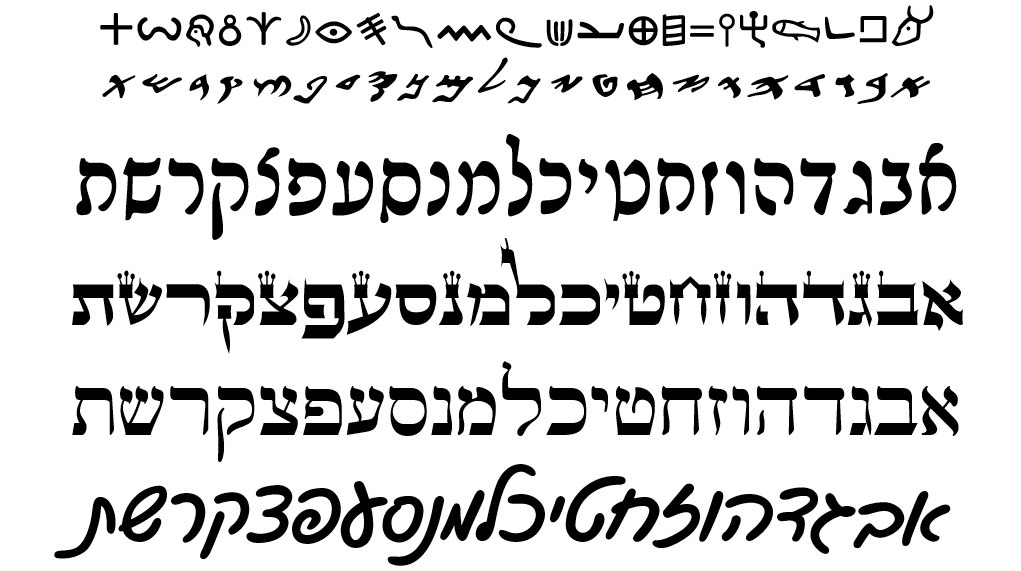
\includegraphics[width=400pt]{images/alephbet_multi} \end{center}

\footnote{This graphic shows the evolution of Hebrew. Top to bottom: proto-canaanite (\textasciitilde1600 BCE), paleo-Hebrew (\textasciitilde900 BCE), Rashi (1500 CE), Ketav Stam (used in Torah scrolls and other formal documents), contemporary block. and contemporary cursive. This course will use contemporary block style. For more history and discussion on the other script forms, see Hebrew Quest, lessons 2-11.}

\hypertarget{seven-practical-points-for-lesson-1}{%
\subsection*{Seven Practical Points for Lesson 1}\label{seven-practical-points-for-lesson-1}}
\addcontentsline{toc}{subsection}{Seven Practical Points for Lesson 1}

\begin{enumerate}
\def\labelenumi{\arabic{enumi}.}
\tightlist
\item
  Memorize the \protect\hyperlink{one_1}{Hebrew Aleph-Bet}
\item
  Understand that \protect\hyperlink{one_2}{Hebrew is written and read from RIGHT to LEFT}
\item
  Identify the group of \protect\hyperlink{one_3}{five letters that have final/Sofit forms}
\item
  Identify the group of \protect\hyperlink{one_4}{six letters that can take a Daghesh Lene}
\item
  Identify the group of \protect\hyperlink{one_5}{four ``guttural'' letters that cause significant changes in spelling and punctuation (and the one additional letter that sometimes acts as a guttural)}
\item
  Differentiate among \protect\hyperlink{one_6}{``look-alike'' letters}
\item
  Note \protect\hyperlink{one_7}{differences between ``seminary'' and ``Sephardic'' pronunciation}
\end{enumerate}

\protect\hyperlink{one_8}{Lesson 1 ACTIVities}

\hypertarget{one_1}{%
\subsection{The Hebrew Aleph-Bet}\label{one_1}}

\begin{center}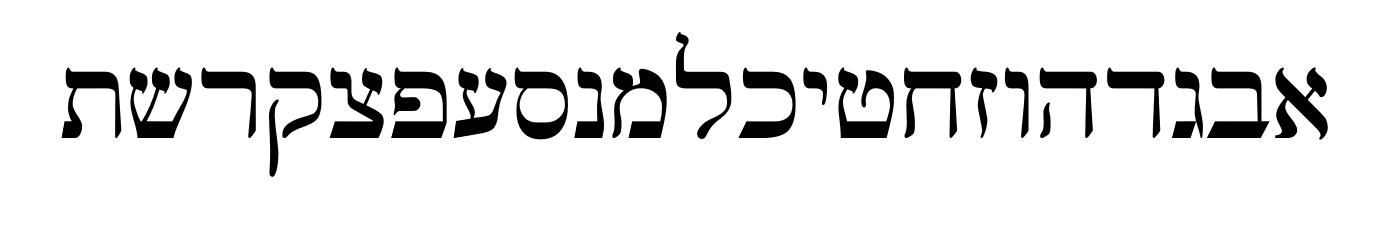
\includegraphics[width=500pt]{images/alephbet} \end{center}

Immediately you will notice that Hebrew GRAMMAR Quest is going to be different from other ``learn Hebrew'' books!

\begin{itemize}
\tightlist
\item
  Almost every other grammar book would start with a lengthy description of each letter, how to write it and how to pronounce it

  \begin{itemize}
  \tightlist
  \item
    But with Hebrew GRAMMAR Quest:
  \end{itemize}
\end{itemize}

\begin{quote}
\emph{We} are not going to teach you the Aleph-Bet - \emph{YOU} are going to teach you the Aleph-Bet!
\end{quote}

\begin{itemize}
\tightlist
\item
  You will accomplish this in Anki. \textbf{You will not want to move on to lesson 2 until you have the Aleph-bet memorized.}
\end{itemize}

Notes:

\begin{itemize}
\tightlist
\item
  All letters you see in the picture of the Aleph-Bet above are classified as ``consonants''

  \begin{itemize}
  \tightlist
  \item
    Whereas English has the vowel letters (A, E, I, O, U) as a core part of the Aleph-Bet, Hebrew treats vowels differently
  \item
    We'll see more in the next lesson
  \end{itemize}
\item
  This would be a great time to review those introductory lessons in Hebrew Quest

  \begin{itemize}
  \tightlist
  \item
    Practical teaching on how to write the letter
  \item
    Spiritual insights - what the letter teaches us
  \end{itemize}
\end{itemize}

\hypertarget{one_2}{%
\subsection{Hebrew is written and read from RIGHT-to-LEFT}\label{one_2}}

\begin{center}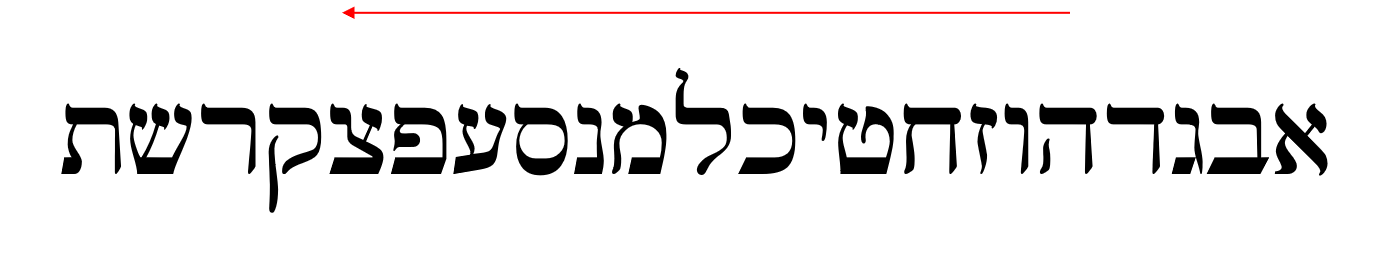
\includegraphics[width=400pt]{images/right_to_left} \end{center}

Note the front of a Hebrew book is in the same location as the back of an English book:

\begin{center}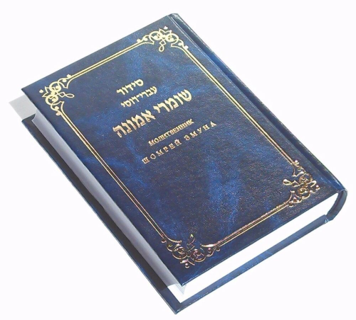
\includegraphics[width=150pt]{images/hebrewbook} \end{center}

\begin{itemize}
\tightlist
\item
  To our western eyes, this looks ``backwards'' (but Israelis would say \emph{we} are reading backwards!)
\item
  When reading Hebrew, always start at the ``back'' and go from RIGHT to LEFT
\end{itemize}

\hypertarget{one_3}{%
\subsection{Five letters have final (``sofit'') forms}\label{one_3}}

\begin{center}
\includegraphics[width=500pt]{images/kimnepatz} \end{center}

\begin{itemize}
\tightlist
\item
  Hebrew does not have capital letters the way English does, but it does have a generally similiar concept
\item
  Certain letters take what are called ``Final'' or ``Sofit'' forms when they appear at the END of a word

  \begin{itemize}
  \tightlist
  \item
    Those letters are in red text above
  \item
    \emph{Sofit} is just the Hebrew word for final
  \end{itemize}
\item
  The names of these letters is quite simple

  \begin{itemize}
  \tightlist
  \item
    Take the letter Kaf כּ, which is the first letter in the Aleph-bet with a sofit form
  \item
    The final form is simply named Kaf Sofit ך (or ``final kaf''). Same for Mem מ and Mem sofit ם and so on\footnote{``Final Kaf'', ``Final Mem'', etc., are also terms you may hear.}
  \end{itemize}
\item
  The five letters that have these forms are the letters, kaf, mem, nun, pei and Tsaddi: ך ם ן ף ץ
\item
  You can remember the acronym, KiMNePaTZ, which is the made-up word you get when you string the five letters in a row
\item
  The KiMNePaTZ sofit forms can look like other letters - your Anki work will give you practice with identifying look-alike letters
\end{itemize}

\hypertarget{one_4}{%
\subsection{Six letters take a ``Daghesh Lene''}\label{one_4}}

\begin{center}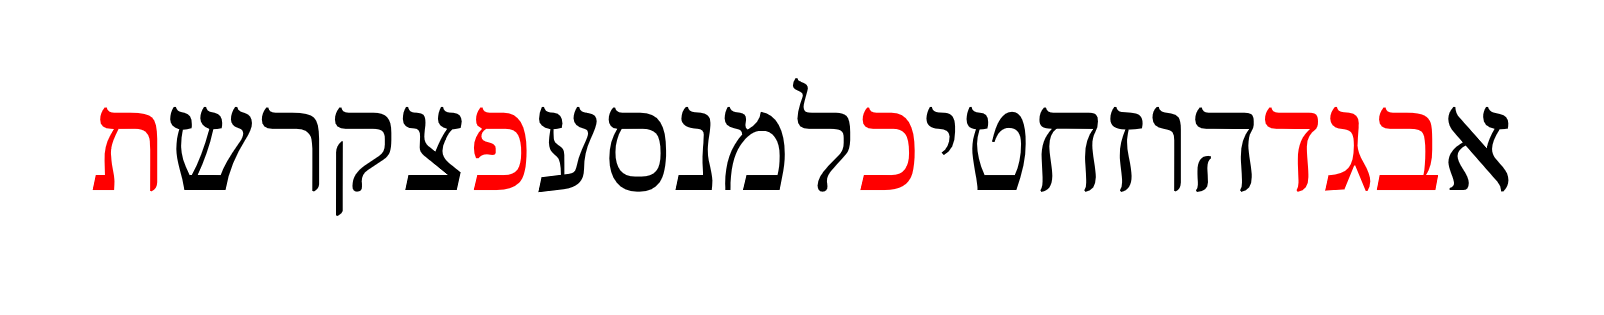
\includegraphics[width=500pt]{images/bgdkpt} \end{center}

\begin{itemize}
\tightlist
\item
  The next sub-group of letters you need to study are the ``BeGaD Kephat'' letters\footnote{See also Lesson 3 of Hebrew Quest}
\end{itemize}

\begin{center}
\includegraphics[width=200pt]{images/bdgkpt_with_lene} \end{center}

\begin{itemize}
\tightlist
\item
  The red dot in the above letters is called a \textbf{DAGHESH LENE}

  \begin{itemize}
  \tightlist
  \item
    It is inserted into the middle of the consonant which makes the pronunciation hard if present, or soft if not present
  \item
    This ONLY to Bet - Gimmel - Dalet - Kaf - Pei - and Tav - we call then ``BeGaD KePHaT'' letters because that's what you get when you string the six letters together
  \item
    Only these six can take a Daghesh Lene\footnote{If you see a dot in a letter other than these six, then you know it can't be a Daghesh Lene}
  \end{itemize}
\item
  At one time all six of these letters had different pronunciation - a hard form and a soft form

  \begin{itemize}
  \tightlist
  \item
    Today only three do: \textbf{בּ כּ פּ}
  \item
    Since the letters without the Daghesh Lene want to be ``lazy'' - for example a weak `v' instead of a strong `b'- our mnemonic for these is ``BuCK uP! You Lazy Letters!''\footnote{You will learn the specific differences in your Anki work for this lesson.}
  \end{itemize}
\end{itemize}

\begin{center}
\includegraphics[width=200pt]{images/buckup} \end{center}

\begin{itemize}
\tightlist
\item
  When will you see a בגד כפת letter with and without the Daghesh Forte?

  \begin{itemize}
  \tightlist
  \item
    There is a rule: A Daghesh Lene is not used whenever the BDGKPT letter follows a Vowel
  \end{itemize}
\end{itemize}

We'll dig deeper into the Daghesh Lene, and its twin, the Daghesh Forte, over the next few lessons.

\hypertarget{one_5}{%
\subsection{Four letters are classified as guttural consonants (and one is a sometimes-guttural)}\label{one_5}}

\begin{center}
\includegraphics[width=500pt]{images/gutturals} \end{center}

\hypertarget{knowing-the-gutturals-and-how-they-behave-will-turn-out-to-be-one-of-the-most-important-facets-of-hebrew-grammar}{%
\subsubsection*{Knowing the gutturals and how they behave will turn out to be one of the most important facets of Hebrew grammar}\label{knowing-the-gutturals-and-how-they-behave-will-turn-out-to-be-one-of-the-most-important-facets-of-hebrew-grammar}}
\addcontentsline{toc}{subsubsection}{Knowing the gutturals and how they behave will turn out to be one of the most important facets of Hebrew grammar}

\begin{itemize}
\tightlist
\item
  Gutturals are everywhere

  \begin{itemize}
  \tightlist
  \item
    We like to say that the gutturals will be our `problem children' because they tend not to play nice with the other Hebrew rules
  \end{itemize}
\item
  There are four proper gutturals Aleph, Hei, Chet, and Ayin (in red above)
  *The letter Resh ר (in orange above) is not formally a guttural; but since it can't decide whether to behave or not, it is often grouped in as a guttural

  \begin{itemize}
  \tightlist
  \item
    The good news is this bad-boy behavior of the gutturals and Resh is entirely predictable
  \item
    We will learn this over the next few lessons (and indeed, the rest of the course)
  \item
    For now just memorize the four guttural consonants in red, and Resh, the sometimes-guttural-like letter in orange.
  \end{itemize}
\end{itemize}

\hypertarget{one_6}{%
\subsection{Look out for look-alike Letters}\label{one_6}}

\begin{center}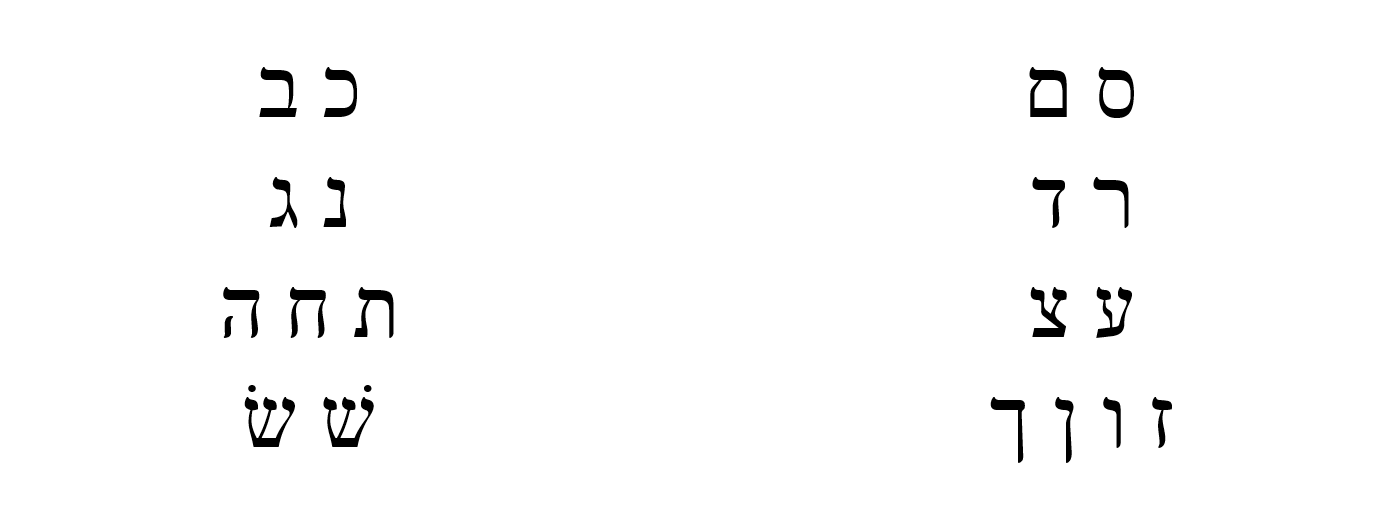
\includegraphics[width=400pt]{images/lookalikes} \end{center}

\begin{itemize}
\tightlist
\item
  Hebrew has many letters that can look similar, especially to someone just learning the Aleph-bet

  \begin{itemize}
  \tightlist
  \item
    The Anki deck will give you practice on distinguishing these.
  \item
    Also, in Hebrew Quest, when Izzy reviewed the Aleph-Bet in lessons 2-11, he also talked about each letter's ``twin'' and how to spot the difference
  \item
    If it's been a while, or if this is new to you, you might want to revisit those letter lessons.
  \end{itemize}
\end{itemize}

\hypertarget{one_7}{%
\subsection{Sephardic vs ``Seminary'' Pronunciation}\label{one_7}}

\begin{center}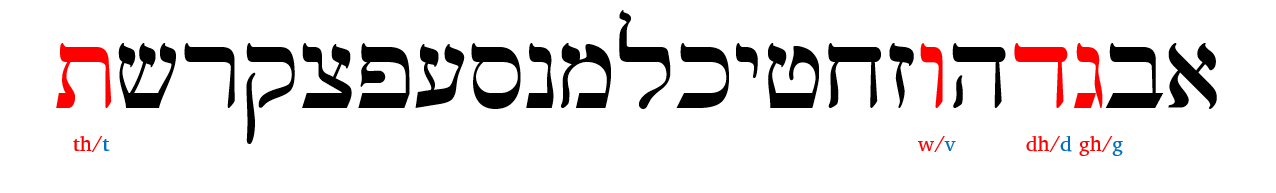
\includegraphics[width=500pt]{images/vav} \end{center}

\begin{itemize}
\tightlist
\item
  There are some notable differences between what we might call academic or ``seminary'' Hebrew and ``real-world'' Hebrew.

  \begin{itemize}
  \tightlist
  \item
    Real-world Hebrew is based on Sephardic pronunciation\footnote{``Seminary Hebrew'' is a term borrowed from Dr.~John Beckman. We don't say ``Seminary Hebrew'' to be disrespectful; we only mean to differentiate between the two pronunciation types.}
  \end{itemize}
\item
  We've already talked about how only three of the Daghesh Lene letters need to ``buckup''\footnote{With ``Seminary Hebrew'', the ג without the Daghesh Lene receives something like the gh in ``aGHast'' and the ד and ת without the Daghesh Lene are closer to the English th like ``this''.}
\item
  Another difference between Sephardic and Seminary pronunciation is how to pronounce ו

  \begin{itemize}
  \tightlist
  \item
    In academia, the consonant receives the ``w'' sound and is called ``Waw.''
  \item
    In most non-academic circles, it receives the ``v'' sound and is pronounced ``vav''.
  \end{itemize}
\item
  There are also significant differences when it comes to pronouncing vowels, which we will talk about in Lesson 2.
\item
  For the most part, Hebrew GRAMMAR Quest will follow the Sephardic pronunciation
\item
  Some terms like ``Waw consective'' and ``wayyiqtol'' are prevalent in the field of Hebrew Grammar, including modern Bible software (see image).
\end{itemize}

\begin{center}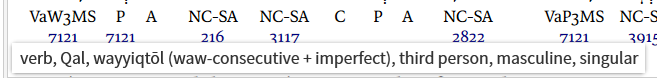
\includegraphics[width=400pt]{images/wayyiqtol} \end{center}

\begin{itemize}
\tightlist
\item
  This course will use ``Adonai'' or ``the LORD'' when we encounter the Tetragramaton\footnote{Pronouncing/writing/transliterating the Holy Name of God tends to be much more common in Christian academic circles. If you were to read ``Basics of Biblical Hebrew'' you would see the name ``Y--w-h'' used frequently. We do know of academians, such as Dr.~John Beckman and Dr.~Robert Cargill, who will use the circumlocution of respect instead of pronouncing the name, so this is not a hard and fast ``seminary'' distinction}.
\end{itemize}

\hypertarget{one_8}{%
\subsection{Lesson 1 ACTIVities}\label{one_8}}

\begin{itemize}
\tightlist
\item
  Physical

  \begin{itemize}
  \tightlist
  \item
    Anki Aerobics

    \begin{itemize}
    \tightlist
    \item
      Vocabulary - Learn (or relearn) the Aleph-Bet with Izzy
    \item
      Grammar - Identify look-alike Hebrew letters
    \end{itemize}
  \item
    \href{https://drive.google.com/file/d/1JcX8kc6e-fKjtzkeE96AwoZFshEpx3ug/view}{Letter Writing worksheet} for practice writing the letters one by one
  \item
    \href{https://drive.google.com/file/d/1mQcP6MMPDU--r374dZii7PxNzyd5NU6F/view?usp=sharing}{Blank writing paper} to practice writing the AlephBet in order. Repeat until you can do it at least five times from memory
  \end{itemize}
\item
  Spiritual

  \begin{itemize}
  \tightlist
  \item
    Anki Aerobics

    \begin{itemize}
    \tightlist
    \item
      Study-Verses - there is no translation yet but we will learn some grammar shorthand that we will use when we get to the study verses
    \end{itemize}
  \item
    \href{https://drive.google.com/file/d/1qcfTKAlTJGChC2eYCMhSbY2w-ibzCcDV/view?usp=sharing}{Ruth Pursuit}\footnote{Click the link (and sign in with a Google account if necessary), then click ``Open with Google Docs'' to highlight the letters.}
  \item
    Instructions:

    \begin{enumerate}
    \def\labelenumi{\arabic{enumi}.}
    \tightlist
    \item
      Identify the four guttural letters (pink)\footnote{The color is to let you know what color the answer key will use, but feel free to highlight in any color, underline, change the font color, or otherwise identify anyway you like.}
    \item
      Identify the one half-guttural (red)
    \item
      Identify the six BeGaD KePHaT letters, both with and without the Daghesh Lene for a total of 12 letters (green)
    \item
      Identify the five final/sofit forms (blue)
    \item
      Identify the remaining letters (yellow)
    \end{enumerate}

    \begin{itemize}
    \tightlist
    \item
      \href{https://drive.google.com/file/d/1vG8hKR50KcB0NclBnRWYPYMCEnobjgLc/view?usp=sharing}{(Ruth Answer Key \#1)}
    \end{itemize}
  \end{itemize}
\item
  Physical - \href{https://docs.google.com/forms/d/e/1FAIpQLSeqHcE8PvfkOYbTu51cNO8sf-ln6CEnRrcTBUxM0EaeojSSsA/viewform}{Quest Quiz \#1}\footnote{Please remember that the Quest Quizzes are intended as a checkpoint of your learning after you have completed the Physical and Spiritual Preparation ACTIVities.}

  \begin{itemize}
  \tightlist
  \item
    After completing all of the other ACTIVities, complete the Quest Quiz to assess your progress
  \end{itemize}
\end{itemize}

\hypertarget{hebrew-vowels}{%
\section{Hebrew Vowels}\label{hebrew-vowels}}

\begin{quote}
And what is required first of all for training men for such a ministry is that the book should be given them in its very words {[}Hebrew, Aramaic, and Greek{]} as it has come from God's hand and in the fullness of its meaning, as that meaning has been ascertained by the labors of generations of men of God who have brought to bear upon it all the resources of sanctified scholarship and consecrated thought.''
---B. B. Warfield\footnote{Warfield, Benjamin Breckenridge. ``The Languages of Pastoral Ministry,'' in Basics of Biblical Hebrew: Grammar, edited by Gary D Pratico and Miles V Van Pelt. Grand Rapids, MI: Zondervan. 2007
  B.B. Warfield was a Presbyterian minister and professor of theology at Princeton Seminary from 1887 to 1921. (\href{https://en.wikipedia.org/wiki/B._B._Warfield}{wikipedia link})}
\end{quote}

\begin{center}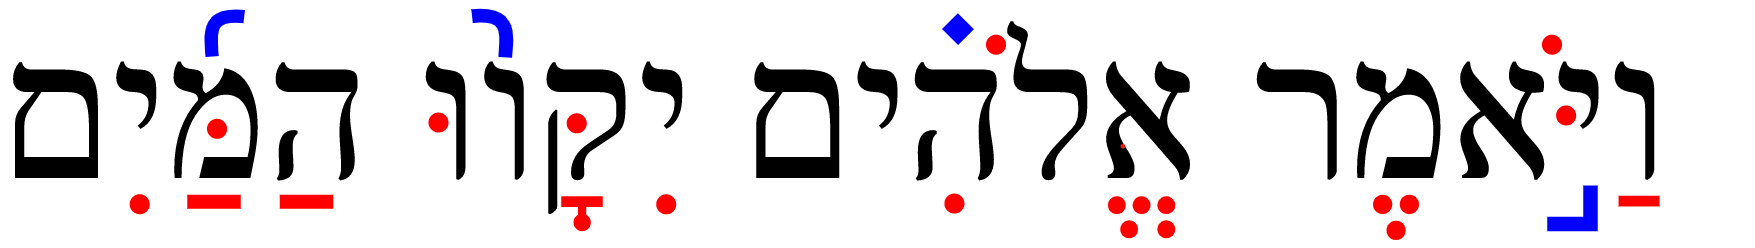
\includegraphics[width=500pt]{images/02.Gen0109} \end{center}

\footnote{As Izzy says in Hebrew Quest, ``Vowels are important.'' On your screen, you see Genesis 1:9. The black font shows the text with no vowels. Over time, vowel notation was developed by the Masorites - these are the symbols in red that are usually under, but sometimes in the middle of, or over the affected consonant to preserve the pronunciation passed down for centuries via the oral tradition. The Hebrew name for these diacritical dots and dashes is \emph{nikudot} . The blue font shows additional cantillation marks, which are used for chanting the verses. These marks also show where the word's accent is.\\
  Image Source: Originally uploaded as en:\url{File:Example} of biblical Hebrew trope.svg on 04:27, 19 November 2006 (UTC) by en:User:SyntaxError55.}

\hypertarget{seven-practical-points-for-lesson-2}{%
\subsection*{Seven Practical Points for Lesson 2}\label{seven-practical-points-for-lesson-2}}
\addcontentsline{toc}{subsection}{Seven Practical Points for Lesson 2}

\begin{enumerate}
\def\labelenumi{\arabic{enumi}.}
\tightlist
\item
  Memorize \protect\hyperlink{two_1}{vowels that are not vowel letters}
\item
  Learn \protect\hyperlink{two_2}{vocal sheva and silent sheva}
\item
  Memorize the \protect\hyperlink{two_3}{vowel letters}
\item
  Meet \protect\hyperlink{two_4}{``defective'' and ``plene'' writing}
\item
  Meet Daghesh Lene's twin, \protect\hyperlink{two_5}{Daghesh Forte}
\item
  Know the \protect\hyperlink{two_6}{rule for a Daghesh Forte}
\item
  Know that the \protect\hyperlink{two_7}{Gutturals and Resh reject Daghesh Forte}
\end{enumerate}

\protect\hyperlink{two_8}{Lesson 2 ACTIVities}

\hypertarget{equipment-check}{%
\subsection*{Equipment Check}\label{equipment-check}}
\addcontentsline{toc}{subsection}{Equipment Check}

\begin{center}
\includegraphics[width=300pt]{images/stopil} \end{center}

Before continuing, can you name the following letters?

\begin{itemize}
\tightlist
\item
  The twenty-two Aleph-Bet letters
\item
  The four BeGaD KePHaT letters
\item
  The five KiMNePaTZ letters
\item
  The four guttural letters and the one sometimes-guttural letter
\end{itemize}

\hypertarget{two_1}{%
\subsection{Vowels that are not vowel letters}\label{two_1}}

\hypertarget{vowels-come-in-three-types-long-short-reduced-vowels-come-in-five-classes-a-e-i-o-u}{%
\subsubsection*{Vowels come in three types: Long, Short, Reduced \textbar{} Vowels come in five classes: A, E, I, O, U}\label{vowels-come-in-three-types-long-short-reduced-vowels-come-in-five-classes-a-e-i-o-u}}
\addcontentsline{toc}{subsubsection}{Vowels come in three types: Long, Short, Reduced \textbar{} Vowels come in five classes: A, E, I, O, U}

Like the Aleph-bet, we are simply going to have to commit the table below to memory

\begin{itemize}
\tightlist
\item
  The letter בּ is provided as a placeholder
\item
  Say the vowel \emph{after} saying the associated consonant\footnote{We will learn that Hebrew loves to break rules. In the next lesson we will learn about an exception to the ``vowel comes after'' rule, called the \emph{furtive patach}.} So the first vowel example is ``baw'' not ``awb''.
\end{itemize}

\begin{center}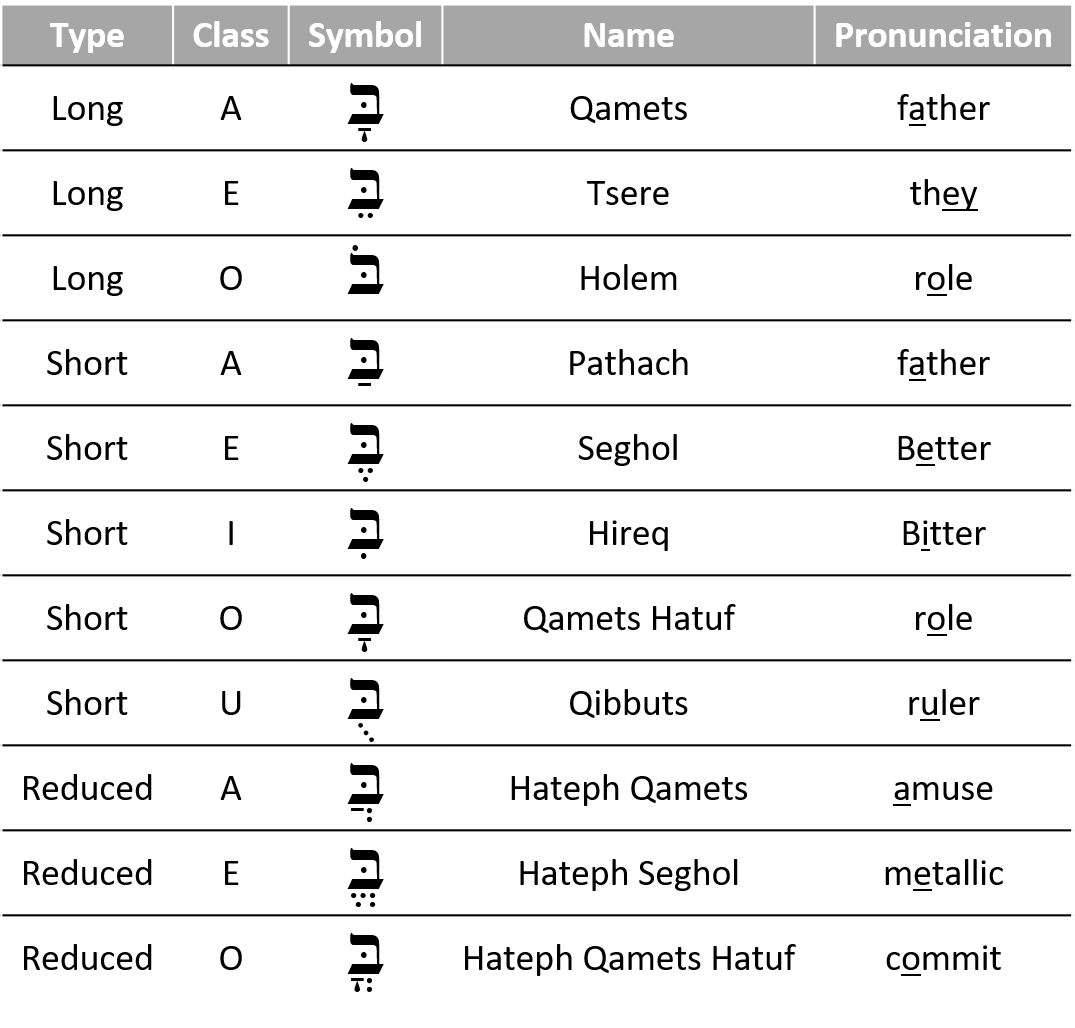
\includegraphics[width=500pt]{images/02.vowels_not_letters} \end{center}

Notes:

\begin{itemize}
\tightlist
\item
  Future lessons will explain the difference between Qamets and Qamets Hatuf
\item
  Only \textbf{gutturals} take the ``Hateph'' vowels - to make it easier, we can pronounce all three Hateph vowels like the A in Amuse
\item
  You might see Kibbuts, Kibbutz, Qibbutz, and Qibbuts used interchangeably
\end{itemize}

\hypertarget{two_2}{%
\subsection{Vocal silent sheva}\label{two_2}}

\hypertarget{both-are-written-as-ux5d1ux5bcux5b0-vocal-sheva-is-a-reduced-vowel-silent-sheva-is-not-a-vowel}{%
\subsubsection{Both are written as: בְּ \textbar{} VOCAL Sheva is a REDUCED vowel \textbar{} SILENT Sheva is NOT A Vowel}\label{both-are-written-as-ux5d1ux5bcux5b0-vocal-sheva-is-a-reduced-vowel-silent-sheva-is-not-a-vowel}}

\begin{itemize}
\tightlist
\item
  Vocal Sheva\footnote{Most academic textbooks will use the term ``shewa'' instead of ``sheva''.}

  \begin{itemize}
  \tightlist
  \item
    Only non-gutturals can take a Vocal Sheva
  \item
    Pronounced like the A in Amuse (same as Hateph Pathach)
  \item
    Is a REDUCED Vowel
  \end{itemize}
\item
  Silent Sheva

  \begin{itemize}
  \tightlist
  \item
    Any letter can take a Silent Sheva
  \item
    Silent/ No sound
  \item
    Is NOT A Vowel
  \end{itemize}
\item
  \_Both Sheva mark the \textbf{END} of a syllable
\item
  We will learn how to distinguish between the two kinds of sheva in the next lesson
\end{itemize}

\hypertarget{two_3}{%
\subsection{Vowel letters}\label{two_3}}

\hypertarget{vowel-letters-use-a-consonant-plus-a-nikkud-to-form-a-vowel}{%
\subsubsection*{Vowel letters use a consonant plus a nikkud to form a vowel}\label{vowel-letters-use-a-consonant-plus-a-nikkud-to-form-a-vowel}}
\addcontentsline{toc}{subsubsection}{Vowel letters use a consonant plus a nikkud to form a vowel}

Another table to memorize:

\begin{center}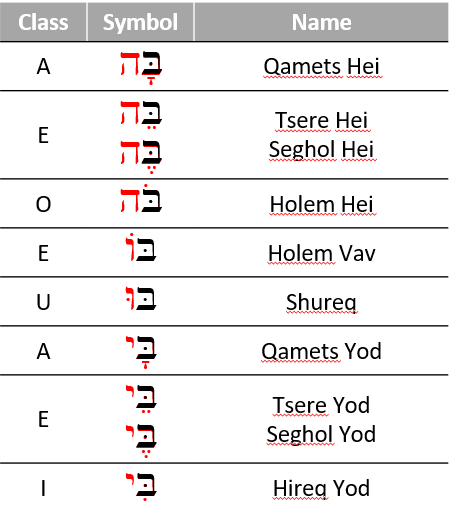
\includegraphics[width=500pt]{images/02.vowels_letters} \end{center}

\begin{itemize}
\tightlist
\item
  Shureq is pronounced like Qibbuts (ruler)
\item
  Hireq Yod is pronounced like the i in machine
\item
  All others are pronounced like their non-vowel-letter counterparts
\item
  Yod and Vav vowels

  \begin{itemize}
  \tightlist
  \item
    These are Long Vowels that do not reduce
  \item
    Therefore they are called ``irreducible (unchangeable) long vowels''\footnote{We'll explain what this means in the next lesson}
  \item
    These occur in the middle or at the end of a word
  \end{itemize}
\item
  Hey Vowels

  \begin{itemize}
  \tightlist
  \item
    Seghol Hei is a short vowel - the other Hei vowels are long
  \item
    Hei vowels \textbf{ONLY} occur at the end of a word
  \item
    Hei vowels are extremely common in Hebrew
  \end{itemize}
\end{itemize}

\hypertarget{two_4}{%
\subsection{``Defective'' and ``plene'' writing}\label{two_4}}

\hypertarget{in-defective-writing-letter-vowels-can-sometimes-drop-their-letter-and-take-on-the-corresponding-non-letter-vowel.-the-meaning-of-word-doesnt-change.}{%
\subsubsection*{In ``defective'' writing, letter vowels can sometimes drop their letter and take on the corresponding non-letter vowel. The meaning of word doesn't change.}\label{in-defective-writing-letter-vowels-can-sometimes-drop-their-letter-and-take-on-the-corresponding-non-letter-vowel.-the-meaning-of-word-doesnt-change.}}
\addcontentsline{toc}{subsubsection}{In ``defective'' writing, letter vowels can sometimes drop their letter and take on the corresponding non-letter vowel. The meaning of word doesn't change.}

This is the word for ``laws'' showing both ``plene'' spelling (left) and ``defective'' spelling (right):

\begin{center}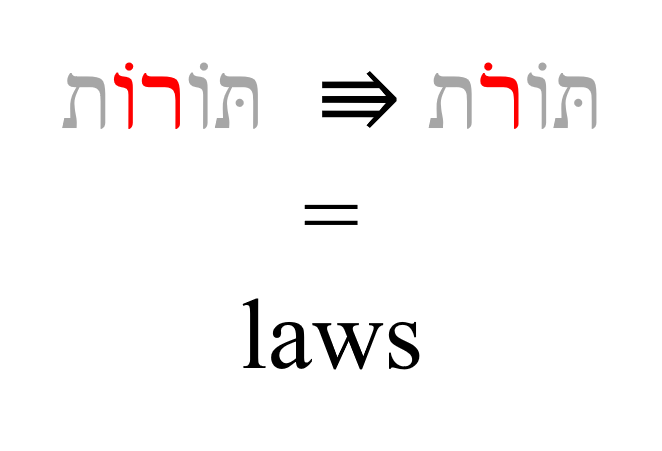
\includegraphics[width=500pt]{images/02.defective} \end{center}

\begin{itemize}
\tightlist
\item
  Three vowel letters can take ``defective'' forms\footnote{``Defective'', in this sense, does not have a negative connotation.}

  \begin{itemize}
  \tightlist
  \item
    Hireq-Yod can drop the Yod and contract to Hireq
  \item
    Holem-vav can drop the Vav and contract to Holem, as in the example above
  \item
    Shuruq, can drop the Vav and it's associated nikkud and contract to Qibbuts
  \end{itemize}
\end{itemize}

Over time, you'll start to develop a mental checklist when you encounter something that doesn't make sense. ``Could this be a defective spelling?'' will be one of those checklist items.

\hypertarget{two_5}{%
\subsection{The Daghesh Forte}\label{two_5}}

\hypertarget{a-daghesh-forte-doubles-the-consonant}{%
\subsubsection*{A Daghesh Forte doubles the consonant}\label{a-daghesh-forte-doubles-the-consonant}}
\addcontentsline{toc}{subsubsection}{A Daghesh Forte doubles the consonant}

Notice the שּׁ in הַשָּׁמַיִם:

\begin{center}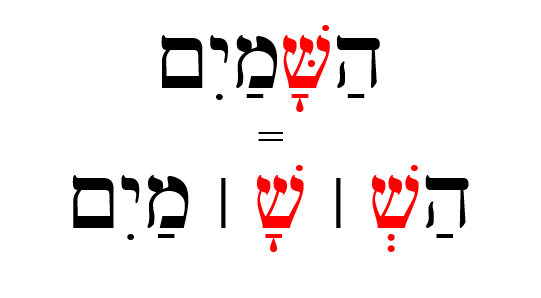
\includegraphics[width=300pt]{images/02.Hashamayim} \end{center}

\begin{itemize}
\tightlist
\item
  Since שׁ is not a בגד כפת letter, we know this \emph{cannot} be a Daghesh Lene, but it is a Daghesh \textbf{Forte}
\item
  The letter with the Daghesh Forte both ends one syllable and begins the next syllable

  \begin{itemize}
  \tightlist
  \item
    If we were to syllabify הַשָּׁמַיִם, it would look something like the bottom line in the picture above (pronounce: hash-sha-mayim\textsuperscript{{[}Mayim is one syllable as we will learn in Lesson 3.{]})}{[}הַשָּׁמַיִם means ``the heavens''. Going forward, we won't always provide a translation for every new word you encounter. It's more important that you focus on the concepts. You will have PLENTY of vocabulary work in Anki!{]}
  \end{itemize}
\item
  A similar word in English might be better = bet \textbar{} ter

  \begin{itemize}
  \tightlist
  \item
    If we were to hypothetically transliterate into Hebrew, it might look like: בּטֶּר*\footnote{The * means this is not a real Hebrew word, but is only given for illustration.}
  \end{itemize}
\item
  Notice the syllable breaks in these words that have a Daghesh Forte:
\end{itemize}

\begin{center}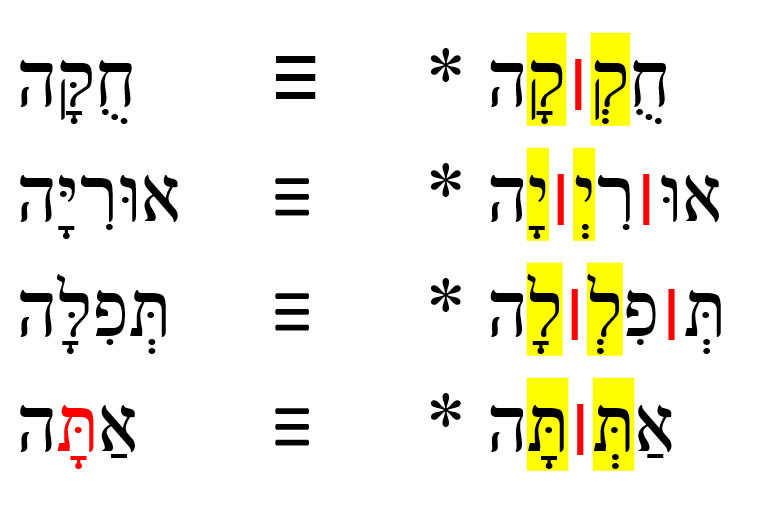
\includegraphics[width=200pt]{images/02.forte} \end{center}

\begin{itemize}
\tightlist
\item
  Any consonant (except for Gutturals and Resh) can take a Dagesh Forte, including בגד כפת letter, which can take either a Daghesh Lene or a Daghesh Forte

  \begin{itemize}
  \tightlist
  \item
    The ``Buck-up'' letters will take the \textbf{hard} pronunciation regardless of a Daghesh Lene or Daghesh Forte

    \begin{itemize}
    \tightlist
    \item
      See the final word אַתָּה in the image above
    \end{itemize}
  \end{itemize}
\end{itemize}

\hypertarget{two_6}{%
\subsection{Daghesh Forte Rule}\label{two_6}}

\hypertarget{a-daghesh-is-a-forte-if-and-only-if-its-preceeded-by-a-vowel-that-is-not-a-sheva.-john-beckman}{%
\subsubsection*{\texorpdfstring{``A Daghesh is a Forte if, and only if, it's preceeded by a vowel\footnote{Remember the rule for the Daghesh Lene? See Lesson 1.4} that is not a sheva.'' ---John Beckman}{``A Daghesh is a Forte if, and only if, it's preceeded by a vowel that is not a sheva.'' ---John Beckman}}\label{a-daghesh-is-a-forte-if-and-only-if-its-preceeded-by-a-vowel-that-is-not-a-sheva.-john-beckman}}
\addcontentsline{toc}{subsubsection}{ ---John Beckman}

That's it. That's the rule\footnote{Strictly speaking, there are exceptions, but you won't encounter them in a first-year Hebrew course}.

Examples:

\begin{itemize}
\tightlist
\item
  אַתָּה = Is the Daghesh preceeded by a vowel that is not a sheva?\footnote{Yes, a pathach. Daghesh Forte}
\item
  בְּרֵאשִׁית = Is the Daghesh preceeded by a vowel that is not a sheva?\footnote{No.~Daghesh Lene}
\item
  עַל־פְּנֵי = Is the Daghesh preceeded by a vowel that is not a sheva?\footnote{No.~Daghesh Lene. The ``hyphen'' looking mark is called a Maqquef. It has the exact same function as the Hyphen does in English.}
\item
  מַבְדִּיל = Is the Daghesh preceeded by a vowel that is not a sheva?\footnote{No, it is preceeded by a sheva. Daghesh Lene.}
\item
  מִתַּחַת = Is the Daghesh preceeded by a vowel that is not a sheva?\footnote{Yes, a Hiriq. Daghesh Forte}
\end{itemize}

\hypertarget{two_7}{%
\subsection{Gutturals and Resh reject Daghesh Forte}\label{two_7}}

\begin{itemize}
\tightlist
\item
  We said in lesson one that the Gutturals don't play nice with the other Hebrew Rules, and this rejection of the Daghesh Forte is one of those ways
\item
  A Hebrew collision like this means something has to give - the gutturals tend to get their way

  \begin{itemize}
  \tightlist
  \item
    A large chunk of Hebrew GRAMMAR Quest will involve how to resolve these situations - more to come!
  \end{itemize}
\end{itemize}

\hypertarget{two_8}{%
\subsection{Lesson 2 ACTIVities}\label{two_8}}

\begin{itemize}
\tightlist
\item
  Physical

  \begin{itemize}
  \tightlist
  \item
    Anki Aerobics

    \begin{itemize}
    \tightlist
    \item
      Vocabulary - Learn (or relearn) the Vowels with Izzy
    \item
      Grammar - More vowel drills. Learn the material in the ``Vocabularly'' deck really well and the ``Grammar'' deck should go smoother.
    \end{itemize}
  \item
    Worksheet

    \begin{itemize}
    \tightlist
    \item
      Practice writing the vowels using the \href{https://drive.google.com/file/d/1ETPKE3u-XGfpNdKmlIr3P_DRbkOOlcI_/view?usp=sharing}{Vowel Writing worksheet/drill} See note\footnote{ignore the ``transliteration'' column. An answer key is on page two. Repeat this worksheet until you can complete it correctly entirely from memory.}
    \end{itemize}
  \end{itemize}
\item
  Spiritual

  \begin{itemize}
  \tightlist
  \item
    Anki Aerobics

    \begin{itemize}
    \tightlist
    \item
      Study-Verses - there is no translation yet but we will learn some very common Hebrew names that we will use when we get to the study verses
    \end{itemize}
  \item
    Ruth Pursuit \href{https://drive.google.com/file/d/1qcfTKAlTJGChC2eYCMhSbY2w-ibzCcDV/view?usp=sharing}{(blank copy)}

    \begin{enumerate}
    \def\labelenumi{\arabic{enumi}.}
    \tightlist
    \item
      Identify the four UNCHANGEABLE LONG vowels that use YOD in Verse 1 (blue)\footnote{In most word processors you won't be able to isolate the vowel to highlight. Just get as close as you can.}\textbar{}
    \item
      Identify the two UNCHANGEABLE LONG vowels that use VAV in Verse 1 (Green)
    \item
      Identify QAMETS HEI in Verse 1. There is a TSERE Hei between Verses 5-10. Can you find it?\footnote{The other vowels that use hei are less common, but we will see them when we discuss verbs.} (Purple)
    \item
      Identify the three LONG vowels in Verse 1 (that are not part of a vowel letter) (pink)\textbar{}
    \item
      Identify three of the five SHORT vowels in Verse 1 (that are not part of a vowel letter)\footnote{We haven't learned to spot Qamets Hatuf yet, and Qibbuts does not appear in this passage} (red)
    \item
      Five the three REDUCED/HATEPHH vowels, including Hateph Qamets Hatuf\footnote{You should be able to make out the word that has the Hateph Qamets Hatuph}. They are in verses 2-4. (grey)
    \item
      One of the more common verbs in the Tanach is \textbf{וַיֹּאמֶר }, which means "(and) he said.

      \begin{itemize}
      \tightlist
      \item
        Vav-Pathach-\textbf{Yod}-Daghesh Forte --וַיּ to start a verb means "And he (did or was something)\\
      \item
        If we change the second consonant from a Yod to a \textbf{Tav}, we get --וָתּ "and \textbf{S}he (did or was something).\\
      \item
        Thus, וַתֹּאמֶר means ``and she said''.\\
      \item
        Challenge: Find the five instances of וַתֹּאמֶר in Ruth Chapter 1\footnote{In at least three of the instances, you should be able to figure out who is speaking.} (yellow)\\
      \end{itemize}
    \end{enumerate}

    \begin{itemize}
    \tightlist
    \item
      \href{https://drive.google.com/file/d/1xtcXRb1PWbt-qkbVWW9yGfkC40_d8gtf/view?usp=sharing}{Ruth Pursuit Answer Key \#2}
    \end{itemize}
  \end{itemize}
\end{itemize}

\hypertarget{Syllabification}{%
\section{Syllabification and Pronunciation}\label{Syllabification}}

\begin{quote}
\end{quote}

\begin{center}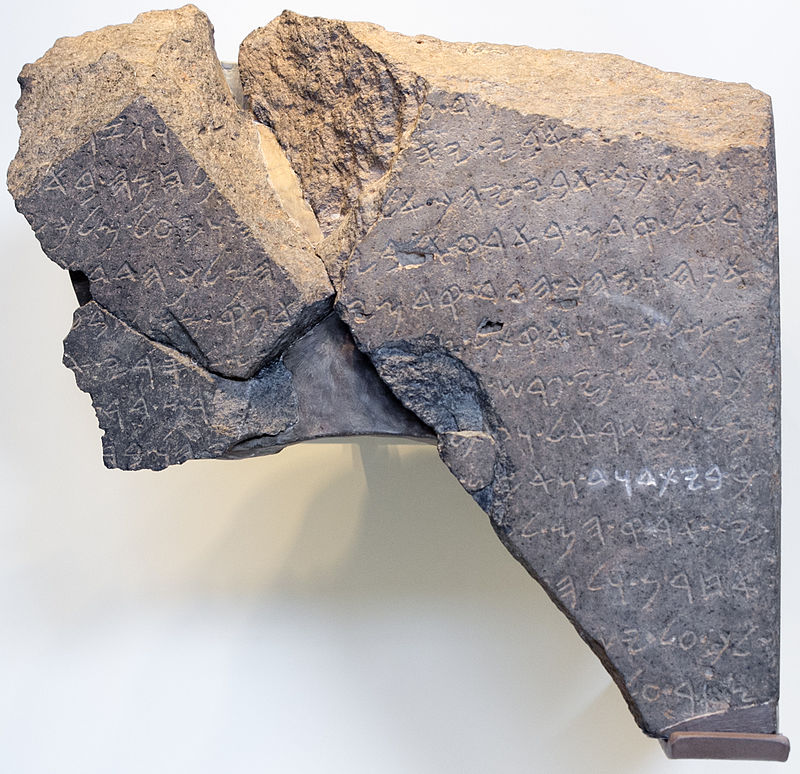
\includegraphics[width=300pt]{images/03.tel-dan} \end{center}

Originally, the Bible and other ancient documents, like the ``Tel Dan Stele'' pictured above\footnote{The Tel Dan Stele was a significant archaeological find of the late 20th century. Written in Aramaic, closely related to Hebrew, the carving dates to the 9th Century BCE. It is notable for containing a reference to the ``house of David'', and is the earliest known extra-biblical reference to King David. Prior to its discovery, many scholars had cast doubt on whether David really existed. It was discovered at the archeological site of ``Dan'' near the Lebanon border in modern Israel. (Photo Credit: By Oren Rozen - Own work, CC BY-SA 4.0, \url{https://commons.wikimedia.org/w/index.php?curid=47055869})}, were written without spaces. In addition to vowels, the ancient scribes and readers organically adopted a system of syllables and accents. They knew where one word ended and another began without needing to write it down.

What we call ``Hebrew grammar'' is truly an exciting journey into the system of spoken and written Hebrew, which had its formation thousands of years ago!

\hypertarget{seven-practical-points-for-lesson-2-1}{%
\subsection*{Seven Practical Points for Lesson 2}\label{seven-practical-points-for-lesson-2-1}}
\addcontentsline{toc}{subsection}{Seven Practical Points for Lesson 2}

\begin{enumerate}
\def\labelenumi{\arabic{enumi}.}
\tightlist
\item
  Learn the two basic concepts of \protect\hyperlink{three_1}{Hebrew Syllables}
\item
  Learn the rules and terminology related to \protect\hyperlink{three_2}{Hebrew Word Accents}
\item
  Know the Three Rules for Recognizing \protect\hyperlink{three_3}{Silent sheva}
\item
  Know the Four RulesRecognizing Vocal sheva: Four Rules Gutturals Reject \protect\hyperlink{three_4}{Vocal Sheva}
\item
  Learn the primary \protect\hyperlink{three_5}{Hebrew Diphthong}
\item
  Understand \protect\hyperlink{three_6}{Vowels and Syllable Preference}
\item
  Learn three simple miscellaneous concepts: \protect\hyperlink{three_7}{Qamets and Qamets Hatuf, Furtive Pathach Quiescent Alef}
\end{enumerate}

\protect\hyperlink{three_8}{Lesson 3 ACTIVities}

\hypertarget{equipment-check-1}{%
\subsection*{Equipment Check}\label{equipment-check-1}}
\addcontentsline{toc}{subsection}{Equipment Check}

\begin{center}
\includegraphics[width=300pt]{images/stopil} \end{center}

Before continuing, can you describe the following concepts?

\begin{itemize}
\tightlist
\item
  The vowels that are not letters, including their type (long, short, reduced) and class (a,e,i,o,u)
\item
  The vowels that are letters, including which are the ``irreducible long'' type
\item
  The difference between a Daghesh Forte and a Daghesh Lene
\end{itemize}

\hypertarget{the-authors-of-basics-of-biblical-hebrew-believe-lesson-3-could-be-the-most-difficult-and-time-consuming-chapter-in-the-book.}{%
\subsubsection*{\texorpdfstring{\textbf{The authors of Basics of Biblical Hebrew believe Lesson 3 could be the most difficult and time-consuming chapter in the book.}}{The authors of Basics of Biblical Hebrew believe Lesson 3 could be the most difficult and time-consuming chapter in the book.}}\label{the-authors-of-basics-of-biblical-hebrew-believe-lesson-3-could-be-the-most-difficult-and-time-consuming-chapter-in-the-book.}}
\addcontentsline{toc}{subsubsection}{\textbf{The authors of Basics of Biblical Hebrew believe Lesson 3 could be the most difficult and time-consuming chapter in the book.}}

If you do not have the vowels and, particularly, the vowel types memorized, this chapter is going to be all the more confusing.

Assuming you've checked your equipment as directed above, and everything is in tip-top shape for your Lesson 3 adventure, just take your time. Work through the written material then do a little Anki work and see if it starts to click.

If not, then come back here and re-read the material again. Then go back to Anki. If you find yourself getting frustrated, take a break and come back to it later. Continue to work through ``the fog.''

You absolutely must have the concepts from this lesson hard-wired before you continue to Lesson 4. The good news is once you get this lesson down, every other lesson is going to be relatively straightforward in comparison to the amount of new concepts you are facing in Lesson 3.

In addition to all of these new concepts, the authors have also seen fit to introduce a full set of vocabulary words AND study verses beginning with Lesson 3. So the overall workload will increase starting with this lesson.

We're praying for you in advance as we compile this section! Now, go climb the mountain!

\hypertarget{three_1}{%
\subsection{Hebrew Syllables}\label{three_1}}

There are two basic concepts when it comes to Hebrew Syllables:

\hypertarget{every-syllable-begins-with-one-consonant-and-has-only-one-vowel}{%
\subsubsection*{Every syllable begins with one consonant and has only one vowel}\label{every-syllable-begins-with-one-consonant-and-has-only-one-vowel}}
\addcontentsline{toc}{subsubsection}{Every syllable begins with one consonant and has only one vowel}

\hypertarget{there-are-only-open-or-closed-syllables}{%
\subsubsection*{There are only open or closed syllables}\label{there-are-only-open-or-closed-syllables}}
\addcontentsline{toc}{subsubsection}{There are only open or closed syllables}

\begin{center}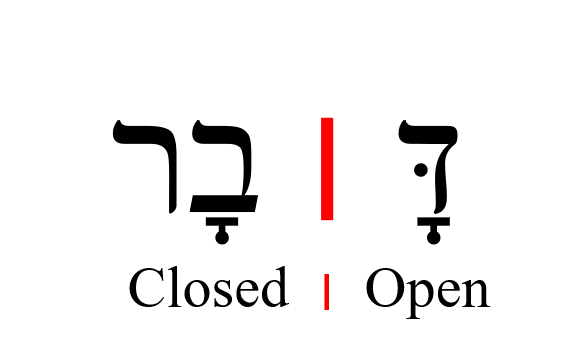
\includegraphics[width=200pt]{images/03.syllable} \end{center}

We see the two basic concepts at play in this simple word (pronounced ``da-var'' and means word, matter, thing):

\begin{itemize}
\tightlist
\item
  The two syllables each begin with a consonant and have one vowel

  \begin{itemize}
  \tightlist
  \item
    דָּ begins with the consonant Dalet, and has one vowel, Qamets

    \begin{itemize}
    \tightlist
    \item
      This is also an example of an ``open'' syllable - open syllables end with a \emph{vowel}, not a consonant
    \end{itemize}
  \item
    בָר begins with the consonant Bet, and has one vowel, also a Qamets

    \begin{itemize}
    \tightlist
    \item
      This is an example of a ``closed'' syllable - closed syllables end with a \emph{consonant}, not a vowel
    \end{itemize}
  \end{itemize}
\item
  If you need to know how many syllables are in a Hebrew word, just count the vowels

  \begin{itemize}
  \tightlist
  \item
    Remember that vowel letters, such as the Hiriq-Yod, and Diphthongs we will later in this lesson count as a single vowel unit
  \end{itemize}
\end{itemize}

\hypertarget{three_2}{%
\subsection{Hebrew Word Accents}\label{three_2}}

\hypertarget{most-frequently-hebrew-words-are-stressed-on-the-last-syllable.}{%
\subsubsection*{Most frequently, Hebrew words are stressed on the last syllable.}\label{most-frequently-hebrew-words-are-stressed-on-the-last-syllable.}}
\addcontentsline{toc}{subsubsection}{Most frequently, Hebrew words are stressed on the last syllable.}

\hypertarget{if-not-then-the-the-accent-will-be-on-the-next-to-last-syllable}{%
\subsubsection*{If not, then the the accent will be on the next-to-last syllable}\label{if-not-then-the-the-accent-will-be-on-the-next-to-last-syllable}}
\addcontentsline{toc}{subsubsection}{If not, then the the accent will be on the next-to-last syllable}

Unlike English, Biblical Hebrew words are never stressed anywhere else\footnote{Modern Hebrew has words (mostly borrowed from other languages) that don't follow this rule}.

\begin{center}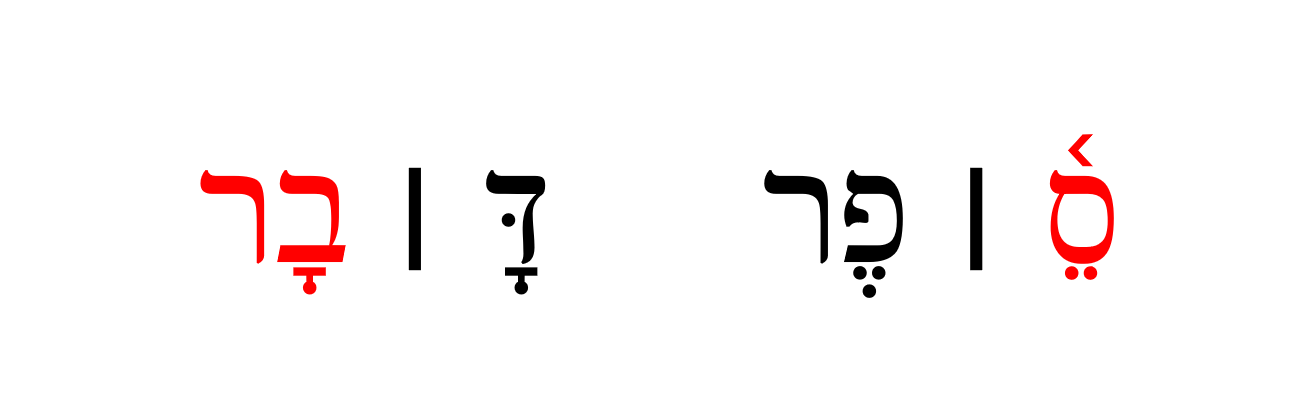
\includegraphics[width=200pt]{images/03.accent_stress} \end{center}

\begin{itemize}
\tightlist
\item
  The word on the left is stressed on the last syllable
\item
  The word on the right (pronounced ``SAY-pher'' or ``SEH-pher'' and means book, scroll, or document) is stressed on the next to last syllable

  \begin{itemize}
  \tightlist
  \item
    Some texts will place a mark over the syllable to be stressed (except when it is on the last syllable)\footnote{Hebrew has a very elaborate system of \href{https://en.wikipedia.org/wiki/Hebrew_cantillation}{cantillation marks} that also serve to indicate where the accent of the word is. are used for chanting and singing. A study of these marks is beyond the scope of this book.}
  \end{itemize}
\end{itemize}

\hypertarget{tonic-pretonic-and-propretonic-syllables}{%
\subsubsection*{Tonic, Pretonic, and Propretonic Syllables}\label{tonic-pretonic-and-propretonic-syllables}}
\addcontentsline{toc}{subsubsection}{Tonic, Pretonic, and Propretonic Syllables}

\begin{itemize}
\tightlist
\item
  We will encounter specific terms for a syllable's position respective to the word's accent
\item
  Let's use the plural of דָּבָר to illustrate: דְּ ׀ בָ ׀ רִים

  \begin{itemize}
  \tightlist
  \item
    The \textbf{Propretonic} syllable is two (or more) steps away from the accent = דְּ

    \begin{itemize}
    \tightlist
    \item
      Notice how the vowel changed from the Qamets in דָּבָר to a Vocal Shewa in דְּבָרִים
    \item
      This vowel shortening of the propretonic syllable is called \emph{Propretonic Reduction} and is extremely common in Hebrew
    \end{itemize}
  \item
    The \textbf{Pretonic} Syllable is the syllable immediately before the accented syllable = בָ
  \item
    The \textbf{Tonic} syllable is the one with the accent = רִים\footnote{Additional info in the textbook that you don't need to know: 1) If there is a syllable AFTER the accented syllable, technically it is called ``Posttonic'' but you will not encounter this term again for the remainder of this course. 2) There is an additional set of terms that signifies a syllable's position irrespective of the accent: \emph{ultima} = the last syllable; \emph{penultima} is the next to last syllable; \emph{antepenultima} is the syllable before the \emph{penultima}}
  \end{itemize}
\end{itemize}

\hypertarget{three_3}{%
\subsection{Silent Sheva}\label{three_3}}

Learn the three rules for differentiating a SILENT Sheva from a Vocal Sheva:

\hypertarget{silent-when-previous-vowel-is-short}{%
\subsubsection*{SILENT when previous vowel is short}\label{silent-when-previous-vowel-is-short}}
\addcontentsline{toc}{subsubsection}{SILENT when previous vowel is short}

\begin{center}
\includegraphics[width=200pt]{images/03.sheva-shortvowel} \end{center}

\hypertarget{silent-when-the-first-of-two-consecutive-shevas-within-a-word}{%
\subsubsection*{\texorpdfstring{SILENT when the first of two consecutive Shevas \emph{within a word}}{SILENT when the first of two consecutive Shevas within a word}}\label{silent-when-the-first-of-two-consecutive-shevas-within-a-word}}
\addcontentsline{toc}{subsubsection}{SILENT when the first of two consecutive Shevas \emph{within a word}}

\begin{center}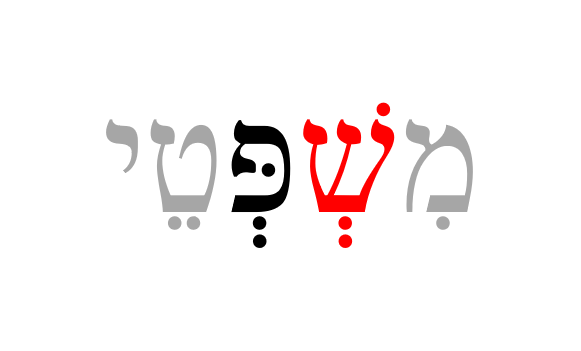
\includegraphics[width=200pt]{images/03.sheva-firstoftwo} \end{center}

\hypertarget{silent-when-at-the-end-of-a-word}{%
\subsubsection*{SILENT when at the end of a word}\label{silent-when-at-the-end-of-a-word}}
\addcontentsline{toc}{subsubsection}{SILENT when at the end of a word}

\begin{center}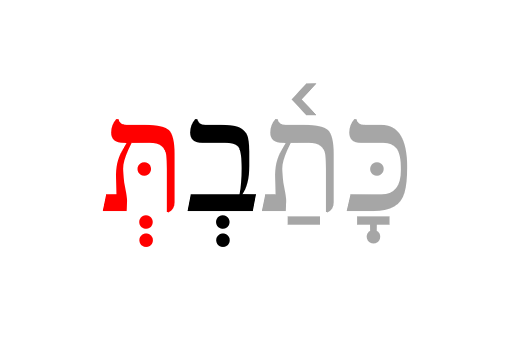
\includegraphics[width=200pt]{images/03.sheva-endofword} \end{center}

\hypertarget{three_4}{%
\subsection{Vocal Sheva}\label{three_4}}

Learn the four rules for differentiating a VOCAL Sheva from a Silent Sheva

\hypertarget{vocal-when-the-initial-sheva-in-a-word}{%
\subsubsection*{VOCAL when the initial Sheva in a word:}\label{vocal-when-the-initial-sheva-in-a-word}}
\addcontentsline{toc}{subsubsection}{VOCAL when the initial Sheva in a word:}

\begin{center}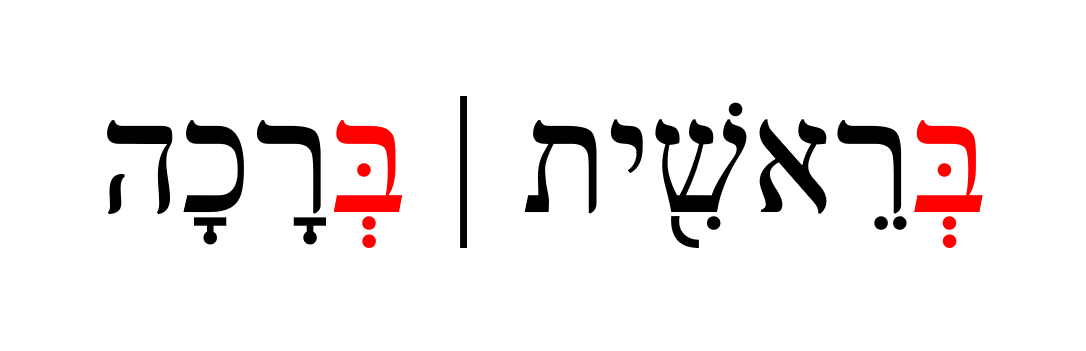
\includegraphics[width=300pt]{images/03.sheva-initialvocal} \end{center}

``buh-rei-sheet'' and ``buh-ra-cha''

\hypertarget{vocal-when-the-second-of-two-consecutive-shevas-within-a-word}{%
\subsubsection*{\texorpdfstring{VOCAL when the second of two consecutive Shevas \emph{within a word}\footnote{A Sheva at the \textbf{end} of a word is \textbf{always silent}, even when it is the second of two consecutive shevas.}:}{VOCAL when the second of two consecutive Shevas within a word:}}\label{vocal-when-the-second-of-two-consecutive-shevas-within-a-word}}
\addcontentsline{toc}{subsubsection}{VOCAL when the second of two consecutive Shevas \emph{within a word}:}

\begin{center}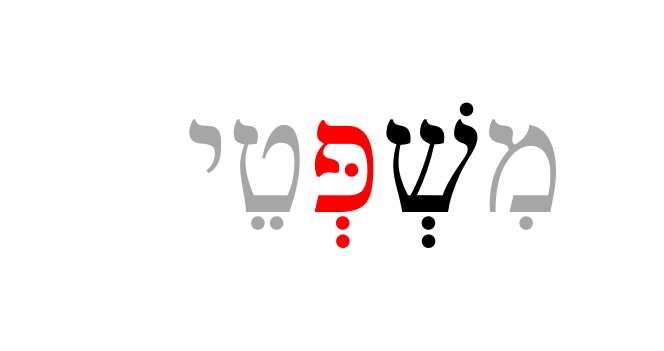
\includegraphics[width=200pt]{images/03.sheva-secondoftwovocal} \end{center}

``mish-puh-tai''

\hypertarget{vocal-when-under-a-daghesh-forte}{%
\subsubsection*{VOCAL when under a Daghesh Forte:}\label{vocal-when-under-a-daghesh-forte}}
\addcontentsline{toc}{subsubsection}{VOCAL when under a Daghesh Forte:}

\begin{center}
\includegraphics[width=200pt]{images/03.sheva-fortevocal} \end{center}

``ham-muh-la-kim''

\hypertarget{vocal-after-an-unaccented-long-vowel}{%
\subsubsection*{VOCAL after an unaccented long vowel:}\label{vocal-after-an-unaccented-long-vowel}}
\addcontentsline{toc}{subsubsection}{VOCAL after an unaccented long vowel:}

\begin{center}
\includegraphics[width=200pt]{images/03.sheva-unaccentedlongvocal} \end{center}

This one may seem random but it is fairly common with long vowels in a propretonic position\footnote{These vowels often but do not always reduce (see section 3.6). Unchangeable long vowels will never reduce.} The word above is not kōṯ-vim but kō-ṯᵉ-vîm.

\hypertarget{three_5}{%
\subsection{Hebrew Diphthong = Accented Pathach-Yod-Hiriq}\label{three_5}}

\begin{center}
\includegraphics[width=200pt]{images/03.diphthong} \end{center}

\begin{itemize}
\tightlist
\item
  The important concept is that the diphthong is one vowel unit, which means it is only one syllable

  \begin{itemize}
  \tightlist
  \item
    The words above are not pronounced ``BUY-it'', but monosyllabic ``BUYIT''; and not ``sh-MY-im'' but ``sh-MYIM''
  \end{itemize}
\end{itemize}

\hypertarget{three_6}{%
\subsection{Vowels and Syllable Preference}\label{three_6}}

\begin{center}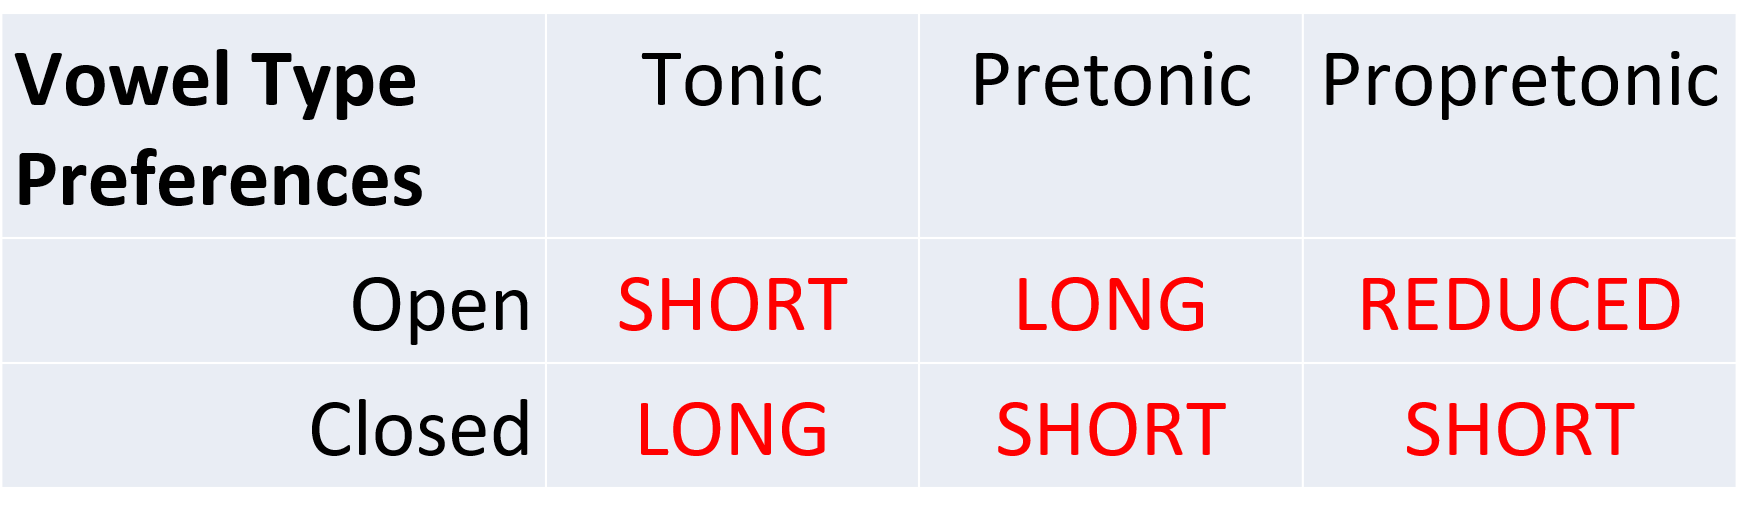
\includegraphics[width=200pt]{images/03.vowelpreferencetable} \end{center}

This table may seem like minutiae, but do yourself a favor: memorize it!

\begin{itemize}
\tightlist
\item
  Open/Propretonic \emph{prefer} reduced vowels but this is why the concept of unchangeable long vowels matter.

  \begin{itemize}
  \tightlist
  \item
    Go back and look at דָּבָר and דְּבָרִים

    \begin{itemize}
    \tightlist
    \item
      The vowel preferance table explains why the vowel under the dalet changes from Qamets in the open pretonic to Vocal Shewa (reduced vowel) in the open propretonic when the plural suffix ``im'' is added
    \end{itemize}
  \item
    As we saw with כֹּתְבִים, propretonic long vowels do not always reduce (and unchangeable long vowels never will)
  \end{itemize}
\end{itemize}

\hypertarget{three_7}{%
\subsection{Qamets Hatuf, Furtive Pathach, Quiescent Alef}\label{three_7}}

These are three miscellaneous but straightforward rules.

\hypertarget{qamets-hatuf-only-occurs-in-a-closed-and-unaccented-syllable}{%
\subsubsection*{Qamets Hatuf ONLY occurs in a Closed AND Unaccented syllable}\label{qamets-hatuf-only-occurs-in-a-closed-and-unaccented-syllable}}
\addcontentsline{toc}{subsubsection}{Qamets Hatuf ONLY occurs in a Closed AND Unaccented syllable}

\begin{center}
\includegraphics[width=200pt]{images/03.qametshatuf} \end{center}

There are many instances where the vowel could be a short qamets-hatuf vowel in a closed syllable, or the long Qamets, A-class vowel in an open syllable. When this ambiguity occurrs, many printings will print a vertical line called a methet. This tells you the vowel is the \textbf{long, a-class}

\hypertarget{furtive-pathach-under-final-ux5d7-or-ux5e2-is-said-before-the-guttural-letter-and-is-not-a-full-vowel}{%
\subsubsection{Furtive Pathach under final ח or ע is said BEFORE the guttural letter and is not a full vowel}\label{furtive-pathach-under-final-ux5d7-or-ux5e2-is-said-before-the-guttural-letter-and-is-not-a-full-vowel}}

\begin{center}
\includegraphics[width=200pt]{images/03.furtivepathach} \end{center}

\begin{itemize}
\tightlist
\item
  The Furtive Pathach is a significant exception to just about everything else we've discussed related to vowels and syllabification:

  \begin{itemize}
  \tightlist
  \item
    The vowel is pronounced \emph{before} the guttural - so the above word is \textbf{Ruach} not ``rucha''
  \item
    The Furtive Pathach is not a full vowel and is counted in syllabification - so the above word is \textbf{Ruach} not ``ru-ach''
  \end{itemize}
\end{itemize}

\hypertarget{quiescent-aleph-is-silent-neither-a-consonant-nor-a-vowel}{%
\subsubsection*{Quiescent Aleph is silent, neither a consonant nor a vowel}\label{quiescent-aleph-is-silent-neither-a-consonant-nor-a-vowel}}
\addcontentsline{toc}{subsubsection}{Quiescent Aleph is silent, neither a consonant nor a vowel}

\begin{center}
\includegraphics[width=200pt]{images/03.quiescentaleph} \end{center}

\begin{itemize}
\tightlist
\item
  When you see an Aleph with no vowels, it is acting as a silent letter

  \begin{itemize}
  \tightlist
  \item
    English has all kinds of silent letters, like the `p' in receipt - the Quiescent Aleph works the same way
  \item
    In terms of syllabification, the Aleph is neither a vowel nor a consonant, so it doesn't count at all - it is just an extra letter
  \end{itemize}
\end{itemize}

\hypertarget{conclusion}{%
\subsection*{Conclusion}\label{conclusion}}
\addcontentsline{toc}{subsection}{Conclusion}

Congratulations for getting this far! This is a tough chapter and, as is our pace, we moved through the ``teaching'' aspects of it quickly to allow you to get started and get learning in Anki.

We realize that there are a lot of heavy concepts you face in this Lesson.

Some of you may try to read this lesson then go do the Anki work (perhaps repeated a few times), and you still aren't getting it. The Fog just isn't clearing. If this is the case, and you want a more in-depth lecture covering this material, we can recommend \href{https://www.youtube.com/watch?v=AY7KAsD4fZg\&feature=youtu.be}{Dr.~John Beckman's hour-long YouTube Lecture on lesson 3}

\hypertarget{three_8}{%
\subsection{Lesson 3 ACTIVities}\label{three_8}}

\begin{itemize}
\tightlist
\item
  Physical

  \begin{itemize}
  \tightlist
  \item
    Anki Aerobics

    \begin{itemize}
    \tightlist
    \item
      Vocabulary - first lesson with a full set of vocabulary words, featuring audio by Izzy!
    \item
      Grammar - All of the concepts you learned in the sections above will be reinforced in Anki

      \begin{itemize}
      \tightlist
      \item
        Like we said in the Equipment Check section, if you absolutely are getting frustrated, take a break or check out the additional in-depth video by Dr.~Beckman
      \end{itemize}
    \end{itemize}
  \end{itemize}
\item
  Spiritual

  \begin{itemize}
  \tightlist
  \item
    Anki Aerobics

    \begin{itemize}
    \tightlist
    \item
      Study-Verses - welcome to our first grouping of study verses, featuring audio by Izzy

      \begin{itemize}
      \tightlist
      \item
        These versus are designed to highlight the vocabularly words learned
      \item
        At first, translation might seem difficult. We'll give you hints as to word meanins along the way until you can build up your vocabulary
      \end{itemize}
    \item
      Over the entire 35 lesson course, you will learn to translate almost 500 Hebrew Verses. The greatest journey begins with a single step. You are now about to take that step!
    \end{itemize}
  \item
    Ruth Pursuit \href{https://drive.google.com/file/d/1qcfTKAlTJGChC2eYCMhSbY2w-ibzCcDV/view?usp=sharing}{(blank copy)}

    \begin{enumerate}
    \def\labelenumi{\arabic{enumi}.}
    \tightlist
    \item
      Identify \textbar{}
    \item
      Identify (Green)
    \item
      Identify (Purple)
    \item
      Identify (yellow)\\
    \end{enumerate}

    \begin{itemize}
    \tightlist
    \item
      {[}Ruth Pursuit Answer Key \#3{]}(
    \end{itemize}
  \end{itemize}
\end{itemize}

\hypertarget{end-of-previewdemo-course}{%
\section*{END OF PREVIEW/DEMO COURSE}\label{end-of-previewdemo-course}}
\addcontentsline{toc}{section}{END OF PREVIEW/DEMO COURSE}

Please email errors, omissions, comments, or suggestions to \href{mailto:holylanguagecourses@gmail.com}{\nolinkurl{holylanguagecourses@gmail.com}}

The anticipated full course availability date is Q2 2021.

Sign up to receive ministry updates and other news at our \href{https://holylanguage.com}{Holy Language Institute website}.

Additional topics to be covered in the full \textbf{\emph{Hebrew GRAMMAR Quest}} book/course:

4 Hebrew Nouns\\
5 Definite Article and Conjunction Vav\\
6 Hebrew Prepositions\\
7 Hebrew Adjectives\\
8 Hebrew Pronouns\\
9 Hebrew Pronominal Suffixes\\
10 Hebrew Construct Chain\\
11 Numerals/counting\\
12 Introduction to Hebrew Verbs\\
13 Qal Perfect - Strong Verbs\\
14 Qal Perfect - Weak Verbs\\
15 Qal Imperfect - Strong Verbs\\
16 Qal Imperfect Weak\\
17 Vav Consecutive\\
18 Qal Imperative\\
19 Pronominal Suffixes on Verbs\\
20 Qal Infinitive Construct\\
21 Qal Infinitive Absolute\\
22 Qal Participle\\
23 Hebrew Syntax\\
24 The Niphal Stem - Strong Verbs\\
25 The Niphal Stem - Weak Verbs\\
26 The Piel Stem - Strong Verbs\\
27 The Piel Stem - Weak Verbs\\
28 The Pual Stem - Strong Verbs\\
29 The Pual Stem - Weak Verbs\\
30 The Hiphil Stem - Strong Verbs\\
31 The Hiphil Stem - Weak Verbs\\
32 The Hophal Stem - Strong Verbs\\
33 The Hophal Stem - Weak Verbs\\
34 The Hithpael Stem - Strong Verbs\\
35 The Hithpael Stem - Weak Verbs

\hypertarget{appendix-appendix}{%
\appendix}


\hypertarget{Anki}{%
\section*{Appendix A: About Anki}\label{Anki}}
\addcontentsline{toc}{section}{Appendix A: About Anki}

\begin{quote}
Anki is like gym equipment for your brain
\end{quote}

\begin{figure}

{\centering 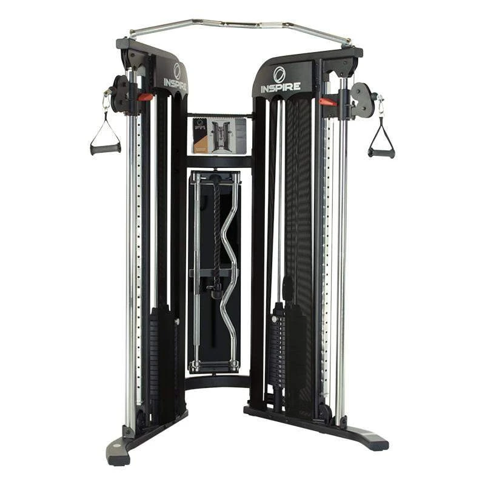
\includegraphics[width=150pt]{images/weight} 

}

\caption{Strength}\label{fig:unnamed-chunk-39}
\end{figure}

\begin{figure}

{\centering 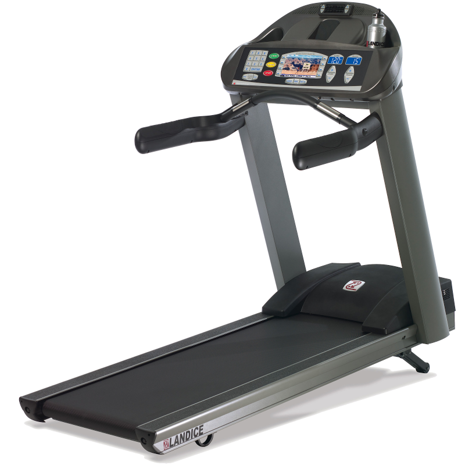
\includegraphics[width=150pt]{images/treadmill} 

}

\caption{Endurance}\label{fig:unnamed-chunk-40}
\end{figure}

If one wants to build strength she might use the weight machine. If one wants to build endurance and overall health, she might use the treadmill. Most people will want to use a combination of both. What does this have to do with Anki (whatever that is)? I'm glad you asked!

What if I told you you could have the equivalent pieces of equipment, only for your brain instead of your physical health and the machine didn't cost you a penny? It's true! That machine is called Anki.

Anki is a tremendous tool for learning and it is where we will be spending the bulk of your time in the course. In fact it has become the ``go to'' for many medical school students for learning all the intricate facts they have to know.

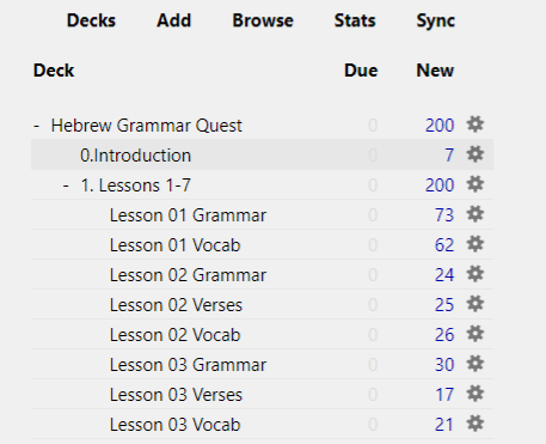
\includegraphics{images/Anki_home_screen.png}

\hypertarget{the-forgetting-curve}{%
\subsection{The Forgetting Curve}\label{the-forgetting-curve}}

\hypertarget{faq}{%
\section*{Appendix B: Questions and Answers about Hebrew GRAMMAR Quest}\label{faq}}
\addcontentsline{toc}{section}{Appendix B: Questions and Answers about Hebrew GRAMMAR Quest}

\hypertarget{difference}{%
\subsection*{What is the difference between Hebrew Quest and Hebrew GRAMMAR Quest?}\label{difference}}
\addcontentsline{toc}{subsection}{What is the difference between Hebrew Quest and Hebrew GRAMMAR Quest?}

\begin{itemize}
\tightlist
\item
  Both courses are born of the same Holy Language Learning philosophy: the optimal way to interact with the Sacred Scriptures is by \emph{doing}
\item
  Hebrew Quest was intentionally designed to get students into Hebrew texts with as little ``grammar'' as possible
\item
  Hebrew GRAMMAR Quest is designed to fill a gap for those students who want to know more about the inner workings of Hebrew, but wish to do so in a fun, low pressure format (as opposed to taking a formal Hebrew course or trying to read an academic-level textbook on their own)
\item
  Also, we know that everyone learns a little differently

  \begin{itemize}
  \tightlist
  \item
    Many are able view the 40 lessons of Hebrew Quest, and they ``get it'' with respect to Hebrew
  \item
    Others may have found themselves getting stuck on the ``grammar'' sections of Hebrew Quest and need some more in-depth grammar preparation before returning to the study passages
  \item
    Still others made it through some or all of Hebrew Quest and just have a desire to know more
  \end{itemize}
\item
  Wherever you find yourself, if you have an interest in digging deeper, you have come to the right place!
\end{itemize}

\hypertarget{do-i-need-to-have-completed-hebrew-quest-before-i-start-hebrew-grammar-quest}{%
\subsection*{Do I need to have completed Hebrew Quest before I start Hebrew GRAMMAR Quest?}\label{do-i-need-to-have-completed-hebrew-quest-before-i-start-hebrew-grammar-quest}}
\addcontentsline{toc}{subsection}{Do I need to have completed Hebrew Quest before I start Hebrew GRAMMAR Quest?}

\begin{itemize}
\item
  Emphatically - \textbf{No!}

  \begin{itemize}
  \tightlist
  \item
    This grammar course starts from the beginning (with learning the Aleph-bet) and assumes no prior knowledge of Hebrew
  \end{itemize}
\item
  With that said, the more of Hebrew Quest you have completed the easier you may find it is to work through the grammar material
\item
  If we were to categorize as ``good'', ``better'', ``best'' in terms of Hebrew Quest completion, here's what we would say:

  \begin{itemize}
  \tightlist
  \item
    \textbf{Good}:

    \begin{itemize}
    \tightlist
    \item
      You have completed some or no Hebrew Quest lessons\\
    \item
      This means that the first three lessons of Hebrew GRAMMAR Quest might take you a little longer, but, once you have that foundation, you'll be up to speed
    \end{itemize}
  \item
    \textbf{Better}:

    \begin{itemize}
    \tightlist
    \item
      You have completed through Hebrew Quest Lesson 12 (the Aleph-bet and Vowels)\\
    \item
      This means the first three lessons will go a little more quickly for you
    \end{itemize}
  \item
    \textbf{Best}:

    \begin{itemize}
    \tightlist
    \item
      You have completed through Lesson 15 (verbs) and beyond
    \item
      This means that more of the concepts presented in Hebrew GRAMMAR Quest will tend be things you have heard before, versus brand new
    \end{itemize}
  \end{itemize}
\end{itemize}

\hypertarget{when-i-complete-this-course-should-i-go-back-and-finish-hebrew-quest}{%
\subsection*{When I complete this course, should I go back and finish Hebrew Quest?}\label{when-i-complete-this-course-should-i-go-back-and-finish-hebrew-quest}}
\addcontentsline{toc}{subsection}{When I complete this course, should I go back and finish Hebrew Quest?}

\begin{itemize}
\tightlist
\item
  \textbf{ABSOLUTELY!}
\item
  In fact, the most logical next step after completing a first-year Hebrew grammar course is to dig into the Scriptures and start reading\\
\item
  Hebrew Quest, starting with Lesson 16 is all about reading Hebrew\footnote{Although, with your deeper knowledge you may be able to go a little faster. If the Hebrew Quest videos are too slow for you, click the ``Settings'' gear icon in the bottom right corner of the video, then click ``Speed'', and then select a faster speed.}
\item
  In other words, Hebrew Quest and Hebrew GRAMMAR Quest compliment each other in a circular (and maybe slightly paradoxical) way:

  \begin{itemize}
  \tightlist
  \item
    The more Hebrew Quest you have completed, the more you will get out of Hebrew GRAMMAR Quest, and
  \item
    The more Hebrew GRAMMAR Quest you have completed, the more you will get out of Hebrew Quest
  \item
    Either way, you can't go wrong!
  \end{itemize}
\end{itemize}

\hypertarget{there-are-many-books-out-there-to-learn-hebrew.-what-makes-hebrew-grammar-quest-different}{%
\subsection*{There are many books out there to learn Hebrew. What makes Hebrew GRAMMAR Quest different?}\label{there-are-many-books-out-there-to-learn-hebrew.-what-makes-hebrew-grammar-quest-different}}
\addcontentsline{toc}{subsection}{There are many books out there to learn Hebrew. What makes Hebrew GRAMMAR Quest different?}

\begin{itemize}
\tightlist
\item
  As we say above, we want students to learn by \textbf{doing}

  \begin{itemize}
  \tightlist
  \item
    While \textbf{Hebrew GRAMMAR Quest} will cover the same concepts as a typical first-year Hebrew textbook, the instructional design team at Holy Language Institute are huge proponents of \emph{active} learning as opposed to passive learning
  \item
    Reading a book is largely a passive activity
  \item
    Therefore, our goal for this book and the accompanying lectures, is to simply provide a quick orientation to the concepts\footnote{In fact, if you're looking for a stand-alone textbook, there is none better than Basics of Biblical Hebrew.}
  \end{itemize}
\item
  Textbooks have their place, but in our view, your ``real'' learning will take place when you complete the ACTIVities (see root of the word ``active'' in there?)

  \begin{itemize}
  \tightlist
  \item
    This is the impetus behind the current ``flipped classroom'' philosophy in traditional education
  \end{itemize}
\end{itemize}

\hypertarget{what-is-a-flipped-classroom}{%
\subsection*{What is a ``flipped classroom''?}\label{what-is-a-flipped-classroom}}
\addcontentsline{toc}{subsection}{What is a ``flipped classroom''?}

\begin{itemize}
\tightlist
\item
  Hebrew GRAMMAR Quest applies concepts from what is called a ``flipped classroom''
\item
  In a traditional classroom, lecture and exams are the priority

  \begin{itemize}
  \tightlist
  \item
    What educators have started to notice was that these two aspects of teaching, though valuable for different reasons, are not when the student's primary learning occurs
  \end{itemize}
\item
  In a flipped classroom, the activities usually thought of as ``homework'' are the priority

  \begin{itemize}
  \tightlist
  \item
    Interactive reading (with note-taking and active-recall), worksheets, and discussion are much better vehicles for learning than a lecture
  \end{itemize}
\item
  Therefore in Hebrew GRAMMAR quest there is an intentional de-emphasis on lectures and exams and an intentional emphasis on activities - in fact to emphasize this emphasis we call these ``ACTIVities''!
\end{itemize}

\hypertarget{what-are-the-activities}{%
\subsection*{What are the ACTIVities?}\label{what-are-the-activities}}
\addcontentsline{toc}{subsection}{What are the ACTIVities?}

We cover all of this in the \protect\hyperlink{preface}{Preface: the philosophy of this book and course} section!

\hypertarget{how-do-i-access-the-anki-deck-or-online-course}{%
\subsection*{How do I access the Anki deck or online course?}\label{how-do-i-access-the-anki-deck-or-online-course}}
\addcontentsline{toc}{subsection}{How do I access the Anki deck or online course?}

\begin{itemize}
\tightlist
\item
  The full program including the Anki package and access to the online course, are available to subscribers of Holy Language Institute
\item
  Login to \url{holylanguage.com}
\item
  Click on the LEARN button then select ``Hebrew GRAMMAR Quest'' \textbf{\emph{(pending development)}}
\end{itemize}

\hypertarget{do-i-need-the-online-course-if-i-have-this-book}{%
\subsection*{Do I need the online course if I have this book?}\label{do-i-need-the-online-course-if-i-have-this-book}}
\addcontentsline{toc}{subsection}{Do I need the online course if I have this book?}

\begin{itemize}
\tightlist
\item
  Strictly speaking, no. This book contains the same links to the same activities as the online course does
\item
  The advantages of the course include all of the ACTIVities in a checklist style format with the ability to quickly determine what you have completed and what you still need to do to complete a given lesson or module
\item
  \textbf{IMPORTANT} - If you wish to be included in our \href{https://holylanguage.com/graduate.html}{Hebrew Quest and Hebrew GRAMMAR Quest graduation process}, where you will receive certificates upon completion of each of the five modules in each course, as well as a congratulatory gift upon completion of the entire course, there are documentation requirements that can \textbf{only} be met by completing the online course
\end{itemize}

\hypertarget{will-i-need-to-buy-anything}{%
\subsection*{Will I need to buy anything?}\label{will-i-need-to-buy-anything}}
\addcontentsline{toc}{subsection}{Will I need to buy anything?}

\begin{itemize}
\tightlist
\item
  \textbf{NO}. Other than being a subscriber to Holy Language Institute, you will not need to purchase anything for this course (unless you want to)
\item
  We would like to disclose that the iOS version of the Anki app requires a one-time purchase through the Apple store of \$25

  \begin{itemize}
  \tightlist
  \item
    Note: Holy Language Institute has nothing to do with this policy and receives nothing should you decide to purchase the app
  \item
    The developers of Anki provide every other platform for free, and say they use the proceeds from the iOS app to fund these other platforms and program enhancements
  \item
    While the price is steep for an app, most online reviews say the cost is justified (a few pennies a day over the course of a year)
  \item
    If you have an Apple device and do not wish to purchase the app, you may use a web-based version of mobile Anki at no charge (you just can't use it offline)
  \end{itemize}
\item
  There are lots of additional resources available that accompany Basics of Biblical Hebrew for free and to purchase - we will incorporate many of the free resources into the online course
\item
  In other words, we have designed this course so that you should not have a need to purchase anything additional by way of learning materials
\item
  With that said, if you wish to purchase \emph{Basics of Biblical Hebrew} or any of the accompanying resources for deeper study, some options are below\footnote{Before purchasing, we would like to make our students aware that the authors of these materials take an academic, as opposed to a reverential approach regarding God's Holy Name and you will see the transliteration of the Tetragrammaton printed on yearly every page. While we believe this is unfortunate and unnecessary, Basics of Biblical Hebrew remains an excellent resource for a in-depth study of first-year Hebrew grammar}

  \begin{itemize}
  \tightlist
  \item
    \href{https://www.amazon.com/gp/product/031053349X/\&tag=holylanginst-20}{Basics of Biblical Hebrew Textbook}
  \item
    \href{https://www.amazon.com/gp/product/0310533554/\&tag=holylanginst-20}{Basics of Biblical Hebrew Workbook}
  \item
    \href{https://www.amazon.com/gp/product/031026295X/\&tag=holylanginst-20}{Basics of Biblical Hebrew Laminated Reference Card}
  \item
    We would appreciate it if you would use one of the affiliate links, which allows Holy Language Institute to receive a small commission
  \end{itemize}
\end{itemize}

\hypertarget{who-will-and-who-might-not-benefit-from-hebrew-grammar-quest}{%
\subsection*{Who will (and who might not) benefit from Hebrew GRAMMAR Quest?}\label{who-will-and-who-might-not-benefit-from-hebrew-grammar-quest}}
\addcontentsline{toc}{subsection}{Who will (and who might not) benefit from Hebrew GRAMMAR Quest?}

\begin{itemize}
\tightlist
\item
  Hebrew GRAMMAR Quest is focused on reading and understanding Hebrew for the English speaker

  \begin{itemize}
  \tightlist
  \item
    If you desire to read the Hebrew Scriptures in the original language and have a greater comprehension of what you read, this course is for you!
  \item
    If one was looking to be a fluent writer or speaker of Hebrew, or teach Hebrew in a formal academic setting, this course probably would not fully meet that person's goals (although it would be a great first step)
  \end{itemize}
\item
  This course focuses on Biblical Hebrew, not Modern Hebrew

  \begin{itemize}
  \tightlist
  \item
    If you are looking to translate ``can you direct me to the railway station?'', we apologize, but this course will not benefit you!
  \end{itemize}
\item
  Hebrew GRAMMAR Quest is designed to be self-directed and (mostly) stress-free

  \begin{itemize}
  \tightlist
  \item
    By design, it does not have the accountability and rigor of a traditional academic program

    \begin{itemize}
    \tightlist
    \item
      By saying it does not have ``academic rigor'', we are \textbf{NOT} saying this course will be easy
    \item
      You will likely spend \emph{many} hours on this course, mostly in Anki
    \item
      We believe it will be a tremendous investment you can make for the kingdom and the impact you can have on others
    \item
      When you start to see your knowledge building up in Anki, we believe you will find it rewarding and perhaps even fun as well
    \end{itemize}
  \item
    Those who seeking more of an academic/seminary type of setting might fare better with a traditional, instructor-led, Hebrew course
  \end{itemize}
\end{itemize}

\hypertarget{what-if-i-am-a-bible-teacher-should-i-take-this-course}{%
\subsubsection*{What if I am a Bible teacher? Should I take this course?}\label{what-if-i-am-a-bible-teacher-should-i-take-this-course}}
\addcontentsline{toc}{subsubsection}{What if I am a Bible teacher? Should I take this course?}

\begin{itemize}
\tightlist
\item
  We believe this course, in conjunction with \textbf{Hebrew Quest}, would prepare a pastor or teacher of a traditional Christian congregation to have a basic understanding of the Hebrew text to be able to exegete and communicate beginning and intermediate level Hebrew/Hebraic concepts to a lay audience

  \begin{itemize}
  \tightlist
  \item
    Additionally, for those who have had first-year Hebrew at seminary (perhaps many years ago) but have struggled to apply knowledge of the original language to their vocation, or for those pastors/teachers who may have never taken a grammar course in Hebrew, \textbf{\emph{our prayer is that this course, along with Hebrew Quest, will give new life to Hebrew application in that person's teaching ministry}}\footnote{This book's author can testify to this!}
  \end{itemize}
\end{itemize}

\hypertarget{about-holy-language-institute}{%
\section*{About Holy Language Institute}\label{about-holy-language-institute}}
\addcontentsline{toc}{section}{About Holy Language Institute}

\begin{center}
\includegraphics[width=500pt]{images/following_yeshua} \end{center}

\textbf{\emph{Jesus is Jewish.}} \{-\}

What if you could get closer to him through Hebrew?

Read on to see what ``Following Yeshua, in a Hebrew way, together'' means to us.

\hypertarget{following-yeshua}{%
\subsection*{Following Yeshua}\label{following-yeshua}}
\addcontentsline{toc}{subsection}{Following Yeshua}

When the first disciples heard ``follow me'', they understood they were being invited into a relationship with this Rabbi from Nazareth. Through this journey of discipleship they would become like him and go on to change the world with him. They knew that following Yeshua was all about knowing Yeshua. That's what our learning experiences are all about.

\hypertarget{in-a-hebrew-way}{%
\subsection*{In a Hebrew Way}\label{in-a-hebrew-way}}
\addcontentsline{toc}{subsection}{In a Hebrew Way}

The disciples of Jesus joined him in reading the Hebrew Bible and praying the Hebrew prayers. That's why this isn't just a language - it's a way of following in the footsteps of the Master, a way of encountering the King of the Jews through the language of his people.

\hypertarget{together}{%
\subsection*{Together}\label{together}}
\addcontentsline{toc}{subsection}{Together}

The men and women who followed Yeshua became a safe and loving community. Same with us! As an organization we're Holy Language ``Institute''. As a community of disciples we're the Holy Language ``Tribe''. Together we're a movement, making disciples and changing the world.

\textbf{\emph{LEARN MORE:}}

\href{https://holylanguage.com/index.html}{Email sign-up}

\href{https://holylanguage.com/subscribe.html}{Become a member} to access the full Hebrew GRAMMAR Quest course, as well as our complete library of teaching materials.

\hypertarget{about-the-designer-of-this-book}{%
\section*{About the designer of this book}\label{about-the-designer-of-this-book}}
\addcontentsline{toc}{section}{About the designer of this book}

\begin{itemize}
\tightlist
\item
  Chris Flanagan has been a member of HLI since 2013 and joined as a ministry volunteer in 2015.
\item
  He has completed Hebrew Quest as a student, which planted a desire to dig deeper into the original languages. He has completed both Hebrew and Greek courses at the seminary level.
\item
  He has worked on a number of projects for HLI from an instructional design standpoint, including leading of ``Hebrew Quest Memrise'' and now ``Hebrew Grammar Quest''

  \begin{itemize}
  \tightlist
  \item
    This work is simply a compilation of many various first-year Hebrew resources, which he has knitted together to present in an original and engaging format
  \item
    For this reason, he likes to refer to himself as the ``designer'' or ``compiler'' of this dynamic Hebrew learning tool, and not the ``author'' of a static book
  \end{itemize}
\item
  Professionally, Chris has worked in the healthcare compliance field for over 30 years
\item
  Personally, Chris is married and has two men in college. He and his wife, Sarah, love to travel, especially to Israel; (which, as you can tell, has inspired the format of each lesson in this book)
\end{itemize}


\includegraphics{images/cf.jpg}

\hypertarget{acknowledgments}{%
\section*{Acknowledgments}\label{acknowledgments}}
\addcontentsline{toc}{section}{Acknowledgments}

All honor and glory to Yeshua, our Lord. שֵׁם יְהוָה אֶקְרָא

Unless, otherwise noted, English Scripture quotations taken from the NASB. Copyright by The Lockman Foundation. Used by permission.

Biblical Hebrew text is courtesy of tanach.us (version 26.0).

Our thanks to Dr.~Gary Pratico and Dr.~Myles Van Pelt for Basics of Biblical Hebrew, the seminary textbook that inspired the format of \textbf{Hebrew Grammar Quest}. We encourage any of our students interested in going deeper with Hebrew grammar to purchase the textbook or any related materials.

Additionally our most grateful thanks to Dr.~John Beckman for making his extensive library of materials to accompany Basics of Biblical Hebrew freely available for reuse under CC-BY-SA.

As applicable:

\begin{itemize}
\tightlist
\item
  Vocabulary portions of this book are derivatives of \href{https://hebrewsyntax.org/bbh2new/00_vocabulary.pdf}{00\_vocabulary.pdf} by John Beckman, used under \href{https://creativecommons.org/licenses/by-nc-sa/4.0/}{CC-BY-SA}.
\item
  Grammar portions of this book are derivatives of \href{https://hebrewsyntax.org/bbh2new/00_study_guide.pdf}{00\_study\_guide.pdf} as well as the ``overhead'' files for each individual chapter (for example \href{https://hebrewsyntax.org/bbh2new/01_overheads_bw.pdf}{Chapter 1-The Hebrew Alephabet}, and so on for each successive chapter) by John Beckman, used under \href{https://creativecommons.org/licenses/by-nc-sa/4.0/}{CC-BY-SA}.
\item
  Study verses portions of this Anki deck are derivatives of \href{https://hebrewsyntax.org/bbh2new/00_workbook_answers.pdf}{00\_workbook\_answers.pdf} by John Beckman, used under \href{https://creativecommons.org/licenses/by-nc-sa/4.0/}{CC-BY-SA}.
\end{itemize}

Finally, we thank YOU for your interest in this course!

\hypertarget{license}{%
\section*{License}\label{license}}
\addcontentsline{toc}{section}{License}

© 2021 Holy Language Institute. All rights reserved.

\begin{figure}
\centering

\includegraphics{images/by-nc-sa.png}
\caption{Creative Commons}
\end{figure}

This work is licensed under the Creative Commons Attribution-NonCommercial-ShareAlike 4.0 International License.

This license is for personal use only. This publication may not be downloaded, redistributed, re-uploaded, published, or used for any other purposes without explicit permission from the copyright holder.

If you received this book and you are not a member of Holy Language Institute, \href{https://holylanguage.com/subscribe.html}{become a member} today! This will give you access to the full Hebrew GRAMMAR Quest course, as well as our complete library of teaching materials.

  \bibliography{book.bib,packages.bib}

\end{document}
